\chapter{Экспериментальные методы измерения коллективной анизотропии}

\section{Эксперимент HADES}

\subsection{Критерии отбора столкновений и рожденных частиц}

В работе приводятся результаты анализа экспериментальных данных, полученные из столкновений ядер Au+Au при энергии $E_{kin}=$1.23$A$~ГэВ а также ядер Ag+Ag при энергиях $E_{kin}=$1.23$A$ и 1.58$A$~ГэВ, полученные на установке HADES.
Всего было проанализировано около 100 миллионов столкновений Au+Au и по 500 миллионов столкновений для Ag+Ag при обеих энергиях.
Для исследования использовались столкновения разделенные по времени и восстановленной вершиной лежащей в области мишени.
Траектории заряженных частиц были отобраны на основании качества аппроксимации трека.
Для отбора первичных частиц использовался критерий на минимальное расстояние между ее траекторией и первичной вершиной. 

Для анализа использовались события столкновений тяжелых ядер, вершина которых лежала в следующих границах: $\sqrt{x_v^2+y_v^2}<3$~мм и $z_v \in (-60, 0)$~мм.
Распределение событий по восстановленной вершине показано на рис.~\ref{fig:hades_vertex}.
Слева представлено распределение восстановленной вершины по оси $z$, справа --- в плоскости $x-y$ для столкновений Au~+~Au при $E_{kin}=1.23A$~ГэВ.
\begin{figure}[ht]
    \begin{center}
        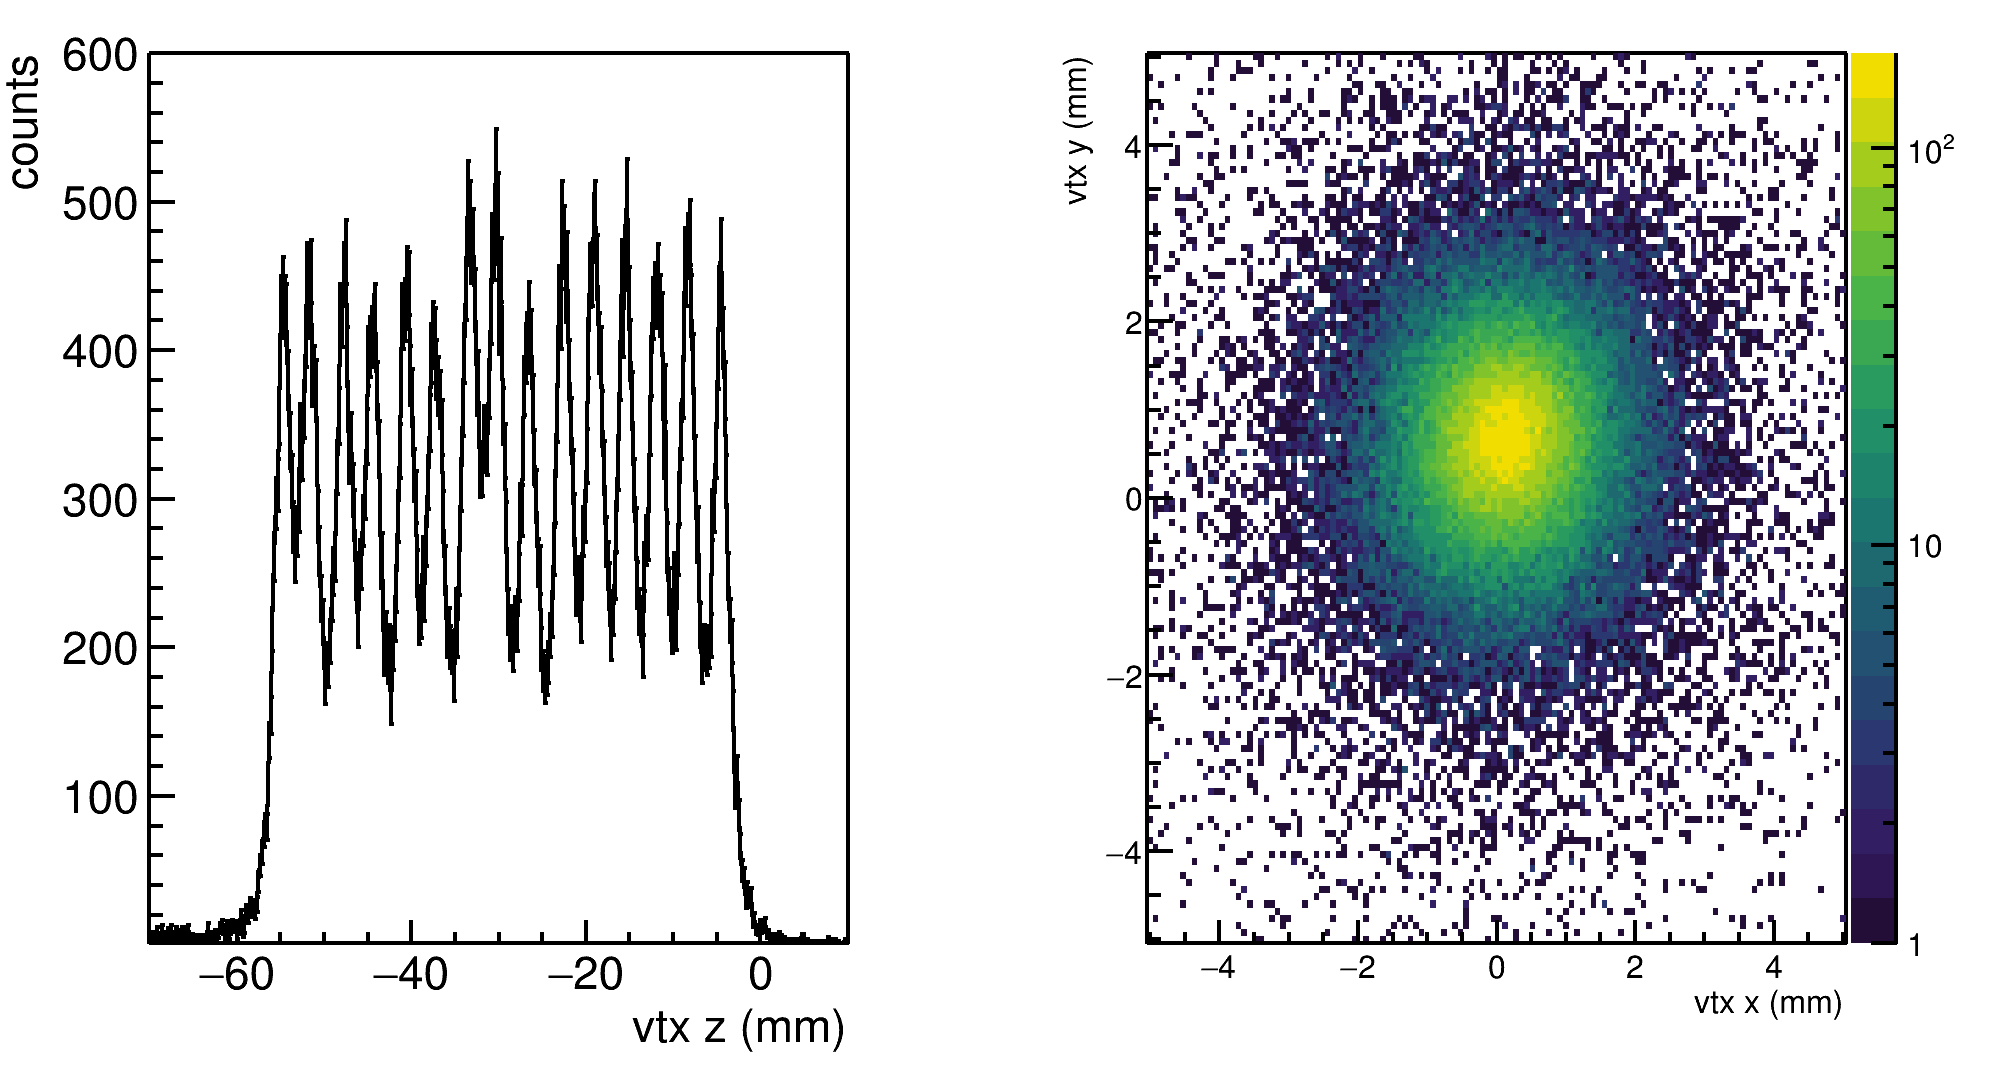
\includegraphics[width=0.95\linewidth]{images/hades_vertex.png}
        \caption{Слева: распределение восстановленной вершины по оси $z$, справа: в плоскости $x-y$ для столкновений Au~+~Au при $E_{kin}=1.23A$~ГэВ.}
        \label{fig:hades_vertex}
    \end{center}
\end{figure}

Для измерения направленного потока использовались траектории заряженных частиц которые были экстраполированы в вершину столкновения.
Траектории которые имели расстояние до восстановленной точки взаимодействия более 10~мм не использовались в анализе.
На рис.~\ref{fig:hades_dca} показано распределение восстановленных траекторий заряженных частиц по расстоянию наименьшего сближения с вершиной столкновения для Au~+~Au при $E_{kin}=1.23A$~ГэВ.
\begin{figure}[ht]
    \begin{center}
        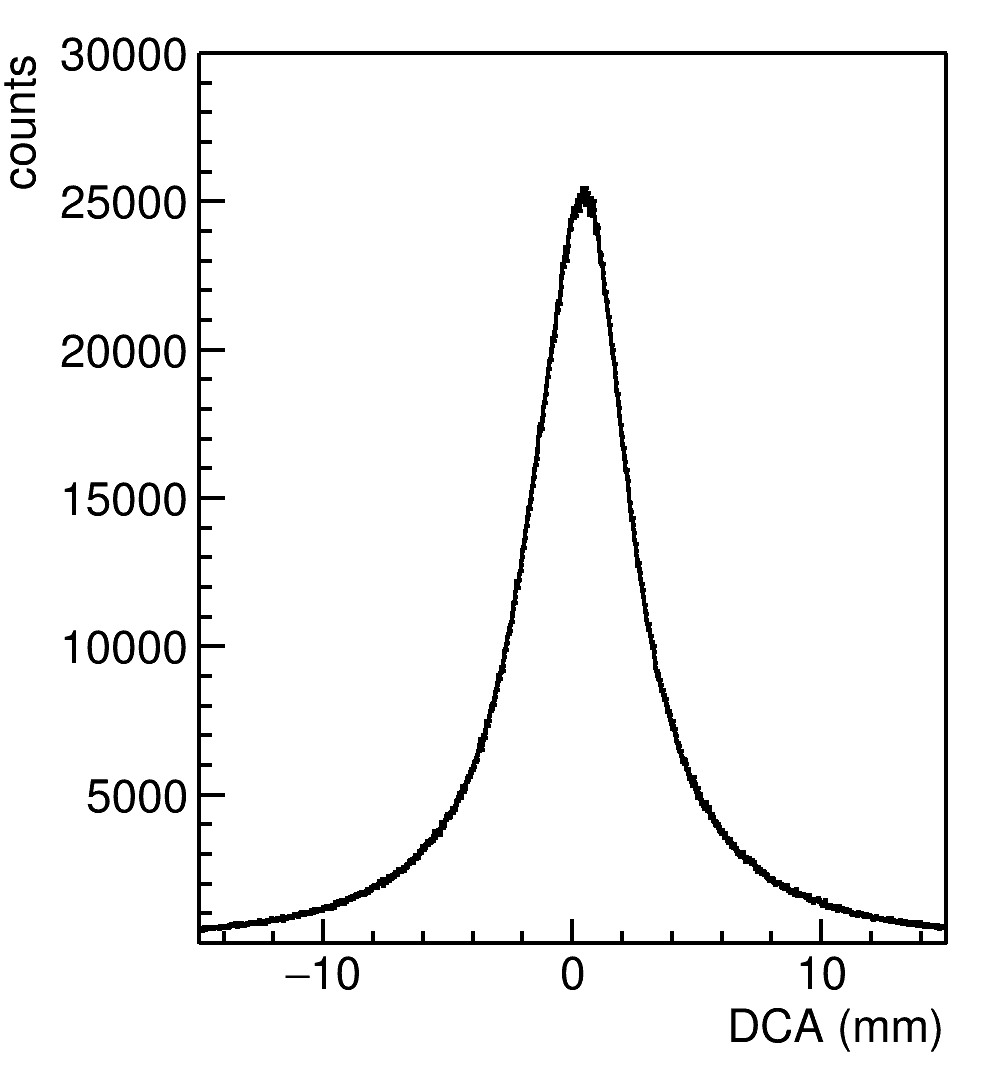
\includegraphics[width=0.55\linewidth]{images/hades_dca.png}
        \caption{Распределение восстановленных траекторий заряженных частиц по расстоянию наименьшего сближения с вершиной столкновения для Au~+~Au при $E_{kin}=1.23A$~ГэВ.}
        \label{fig:hades_dca}
    \end{center}
\end{figure}

\subsection{Определение центральности столкновения}

Центральность столкновений в эксперименте HADES была определена на основе числа срабатываний времяпролетной системы.
Регистрация столкновения выполняется по величине, пропорциональной множественности рожденных в столкновении частиц.
Триггер столкновения вырабатывается при превышении сигналом заданного порога.
Наиболее вероятными являются периферические столкновения, однако в силу малой множественности эти столкновения могут не вырабатывать необходимый сигнал для срабатывания триггера.
Это приводит к тому, что экспериментальное распределение множественности смещается в сторону более центральных столкновений.
Определеные классы центральности по такому распределению множественности тоже будут смещены.
К примеру, на рис.~\ref{fig:hades_multiplicity_comparison} представлено сравнение множественности срабатываний времяпролетной системы TOF+RPC для центрального триггера в столкновениях Au~+~Au при $E_{kin}=1.23$ и Ag~+~Ag при $E_{kin}=1.23$ и $E_{kin}=1.58A$~ГэВ.
Максимальная множественность в столкновениях ядер золота почти в 2 раза превышает максимальную множественность в столкновениях ядер серебра при одной энергии.
Для всех систем и энергий заметен спад в распределении для небольших значений множественности, который объясняется ограниченной эффективностью центрального триггера.
\begin{figure}[ht]
    \begin{center}
        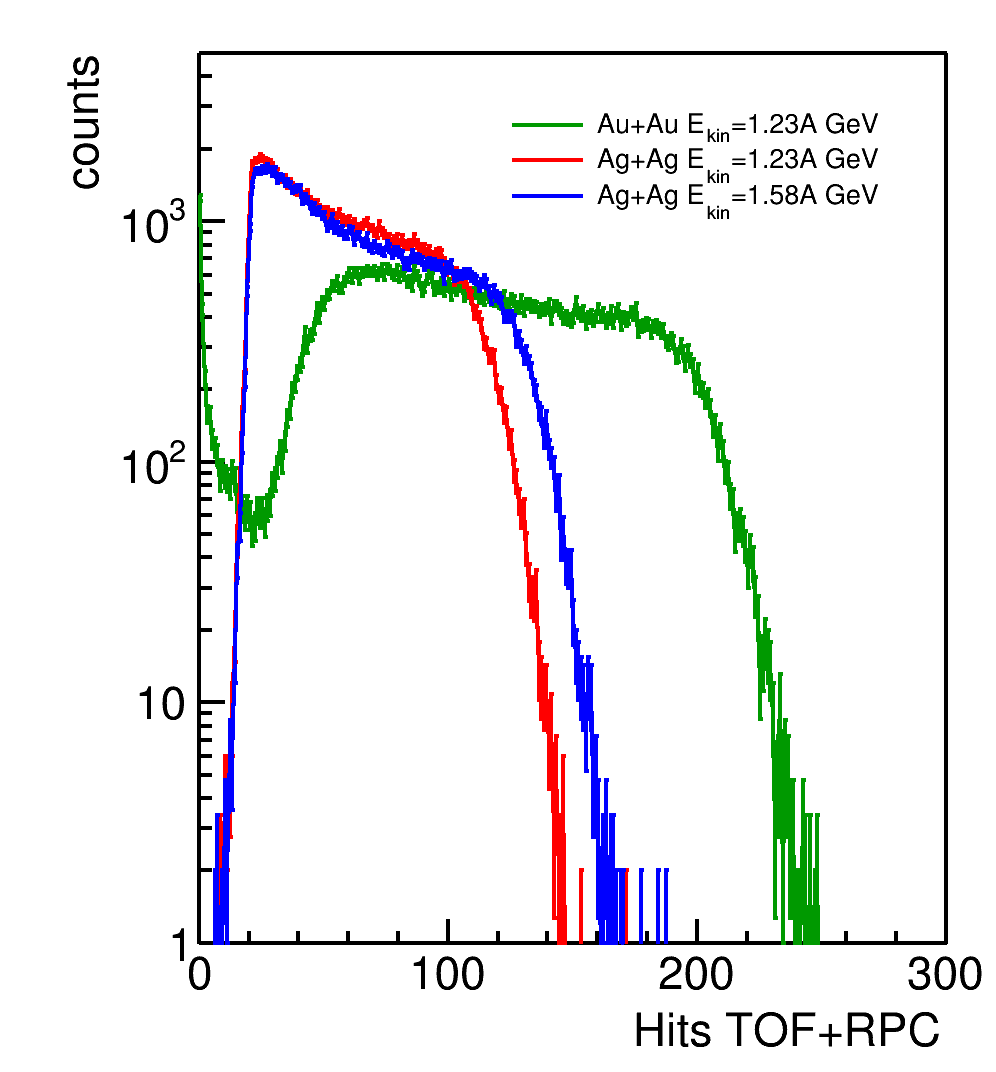
\includegraphics[width=0.55\linewidth]{images/hades_multiplicity_comparison.png}
        \caption{Сравнение множественности срабатываний времяпролетной системы TOF+RPC для центрального триггера в столкновениях Au~+~Au при $E_{kin}=1.23$ и Ag~+~Ag при $E_{kin}=1.23$ и $E_{kin}=1.58A$~ГэВ.}
        \label{fig:hades_multiplicity_comparison}
    \end{center}
\end{figure}
        
Для восстановления истинного распределения множественности с полным сечением неупругого взаимодействия и сопоставления классов центральности со средними значениями геометрических параметров в этих классах использовался метод МК-Глаубера~\cite{HADES:2017def}.
При помощи модели МК-Глаубера (параметры распределения Вудса-Саксона (\ref{eq:woods_saxon}): $R=6.55$~фм и $a=0.52$~фм~\cite{LandoltBornstein2004:sm_lbs_978-3-540-45555-4_81}) разыгрывалось число нуклонов-участников $N_{part}$ и число нуклон-нуклонных столкновений $N_{col}$.
Затем, варьируя параметры отрицального биномиального распределения $f$, $\mu$ и $k$, моделированное распределение множественности подгонялось под экспериментально измеренное распределение числа срабатываний времяпролётной системы TOF+RPC.
Восстановленное распределение множественности из связки МК-Глаубера и отрицательного биномиального распределения было разбито на классы центральности.
В каждом классе центральности из модели МК-Глаубера были извлечены средние значения геометрических параметров.

На рис.~\ref{fig:mc_glauber_auau} слева представлено распределение множественности срабатываений системы TOF-RPC в сеансе Au~+~Au при энергии 1.23$A$~ГэВ. Макрерами разных цветов обозначены данные, собранные с различными триггерами: "min-bais" --- триггер минимального смещения множественности и "central" --- триггер центральных событий.
Красная линия обозначает восстановленное методом МК-Глаубера распределение множественности с полным сечением.
Вертикальные линии обозначают границы классов центральности по множественности.
Для триггера центральных событий (зеленые маркеры) наблюдается хорошее согласие с восстановленной множественностью (красная линия) для классов центральности 0-30\%.
Триггер минимального смещения множественности (синие маркеры) эффективен для классов центральности 0-60\%.
Справа представлено распределение столкновений по множественности и прицельному параметру из модели МК-Глаубера. 
Горизонтальными пунктирными линиями обозначены границы классов центральности.
Для каждого из классов центральности было рассчитано среднее значение прицельного параметра.

\begin{figure}[ht]
\begin{center}
    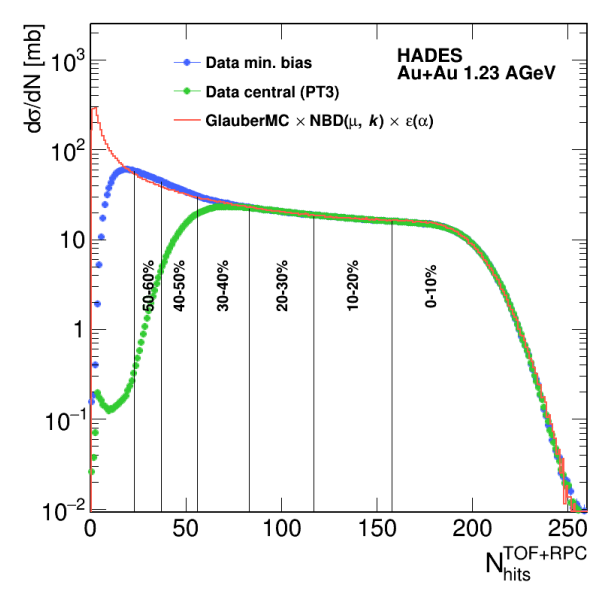
\includegraphics[width=0.45\linewidth]{images/mc_glauber_auau_mult.png}
    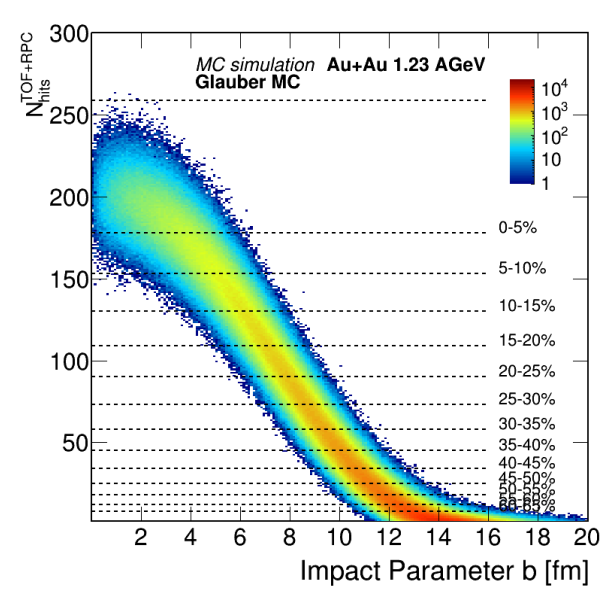
\includegraphics[width=0.45\linewidth]{images/mc_glauber_auau_b_mult.png}
    \caption{Слева: распределение множественности срабатываений системы TOF-RPC в сеансе Au~+~Au при энергии 1.23$A$~ГэВ. Справа: распределение разыгранной множественности методом МК-Глаубера и прицельного параметра для столкновений Au~+~Au при энергии 1.23$A$~ГэВ.}
    \label{fig:mc_glauber_auau}
\end{center}
\end{figure}
    

\subsection{Эффективность реконструкции протонов}

Эффективность реконструкции протонов была рассчитана при помощи Монте-Карло моделирования отклика детектора. 
В качестве входных данных использовалась физическая модель DCM-QGSM-SMM~\cite{Botvina:1994vj, Baznat:2019iom}.
Реалистичный отклик детекторов был смоделирован при помощи программного пакета GEANT3. 
Далее по модели отклика детектора была произведена реалистичная реконструкция.
Эффективность реконструкции определяется формулой:
\begin{equation}
    e(y, p_T) = \frac{ N_{rec}(y,p_T) }{ N_{sim}(y, p_T) },
\end{equation}
где $e(y, p_T)$ --- эффективность реконструкции для данных значений поперечного импульса ($p_T$) и быстроты ($y$), $N_{rec}$ --- число реконструированных частиц, $N_{sim}$ --- число смоделированных частиц.
На рис.~\ref{fig:hades_efficiency} представлена эффективность реконструкции протонов как функция быстроты ($y$) и поперечного импульса ($p_T$) для столкновений Au + Au при энергии $E_{kin}$=1.23$A$~ГэВ (слева), Ag + Ag при энергии $E_{kin}$=1.23$A$~ГэВ (посередине) и $E_{kin}$=1.58$A$~ГэВ (справа).
%
\begin{figure}[ht]
\begin{center}
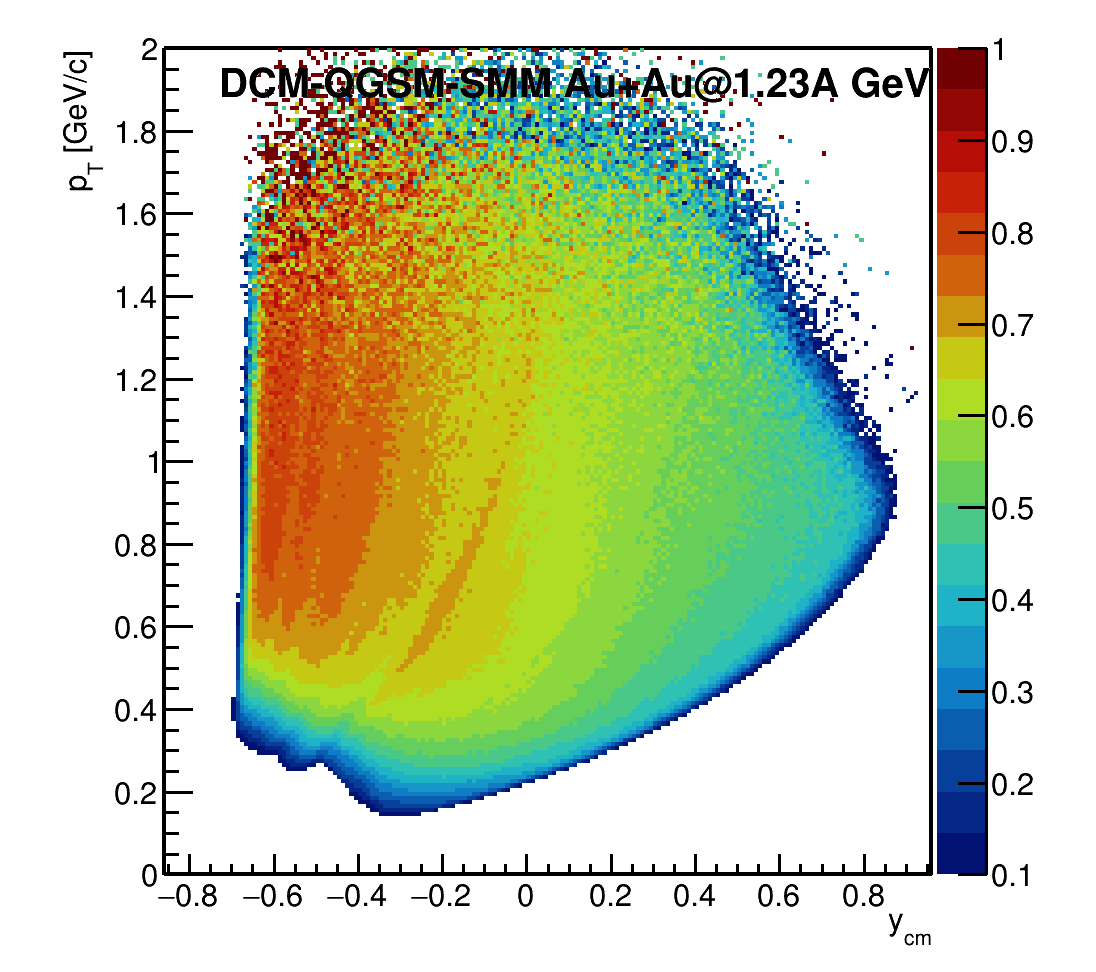
\includegraphics[width=0.3\linewidth]{images/au123_efficiency_y_pT.png}
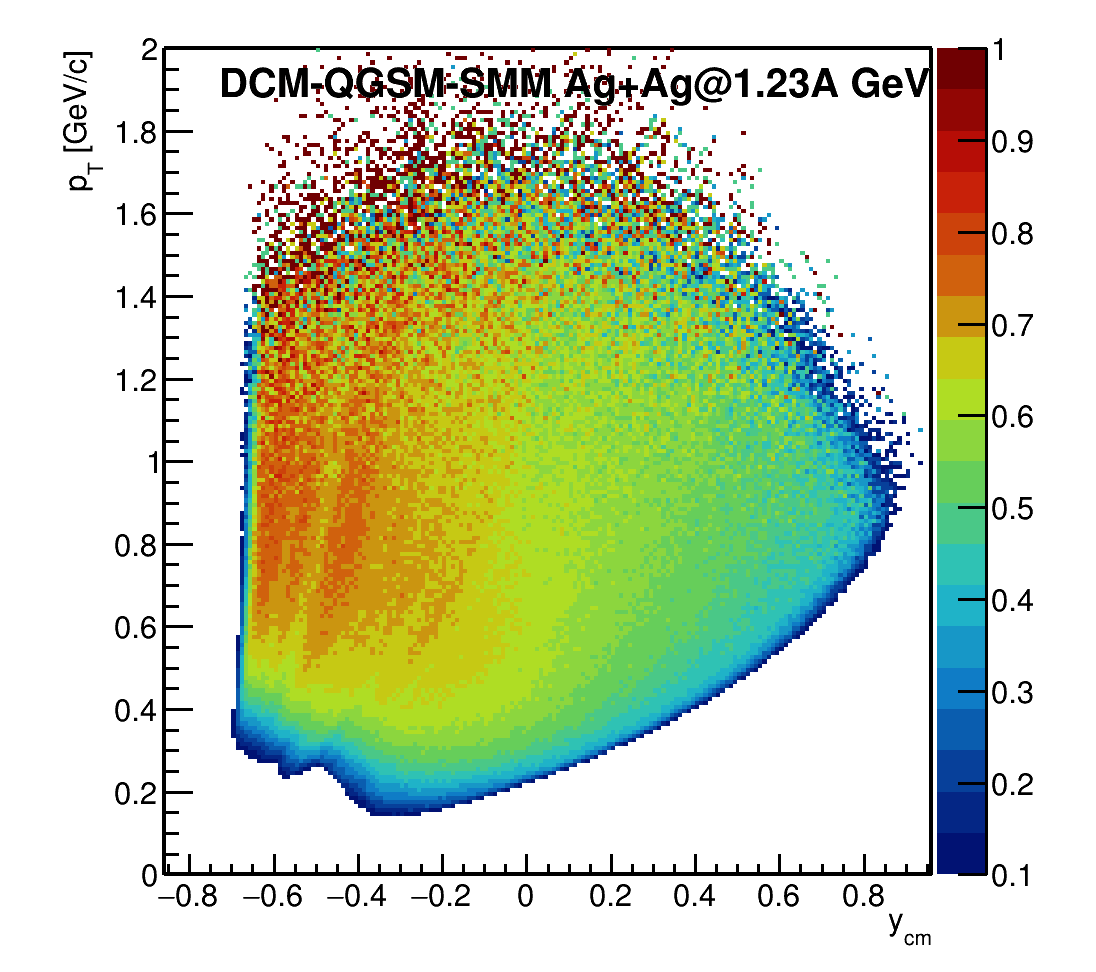
\includegraphics[width=0.3\linewidth]{images/ag123_efficiency_y_pT.png}
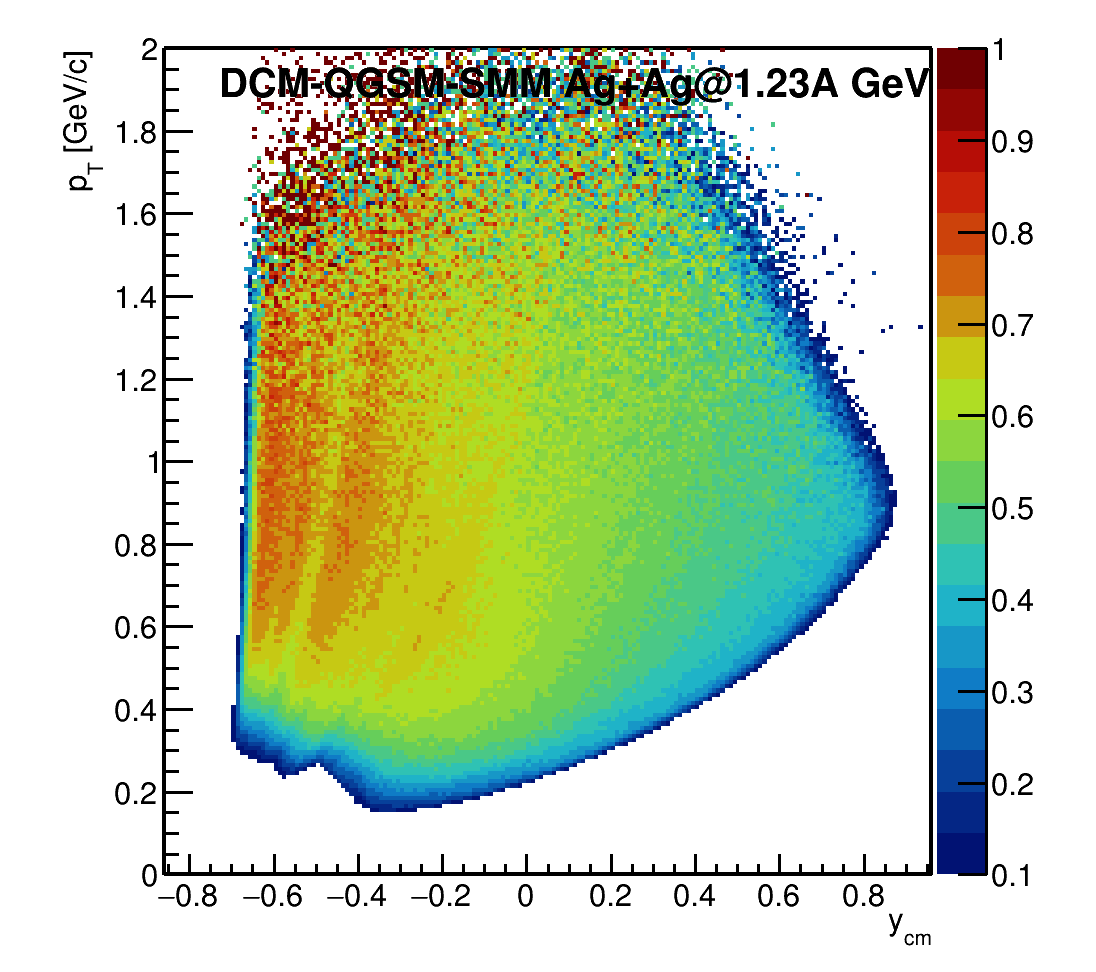
\includegraphics[width=0.3\linewidth]{images/ag158_efficiency_y_pT.png}
\caption{Эффективность реконструкции протонов как функция быстроты ($y$) и поперечного импульса ($p_T$) для столкновений Au + Au при энергии $E_{kin}$=1.23$A$~ГэВ (слева), Ag + Ag при энергии $E_{kin}$=1.23$A$~ГэВ (посередине) и $E_{kin}$=1.58$A$~ГэВ (справа). }
\label{fig:hades_efficiency}
\end{center}
\end{figure}

\subsection{Идентификация протонов времяпролётным методом}

Для измерения времени пролёта, установка HADES оборудована времяпролётными системами TOF и RPC, которые располагаются за трекинговой системой (см. рис.~\ref{fig:hades_bmn_layouts}).
Детектор TOF состоит из сцинтиляционных стержней, ориентированных радиально.
Детекторная подсистема RPC представляет из себя набор резистивных камер.
Идентификация частиц проводилась одновременно времяпролётным методом и по энерговыделению в камерах MDC.
На рис.~\ref{fig:hades_pid} представлено распределение заряженных частиц, зарегистрированных трекинговой системой HADES по относительной скорости $\beta$ и импульсу делённому на заряд $p/q$.
Используя соотношение:
\begin{equation}
    p = \frac{ m\beta }{ \sqrt{1-\beta^2} },
\end{equation}
где $p$ --- импульс частицы, $m$ --- ее масса, $\beta=v/c$, ее относительная скорость, можно рассчитать массу частицы.
%
\begin{figure}[ht]
    \begin{center}
    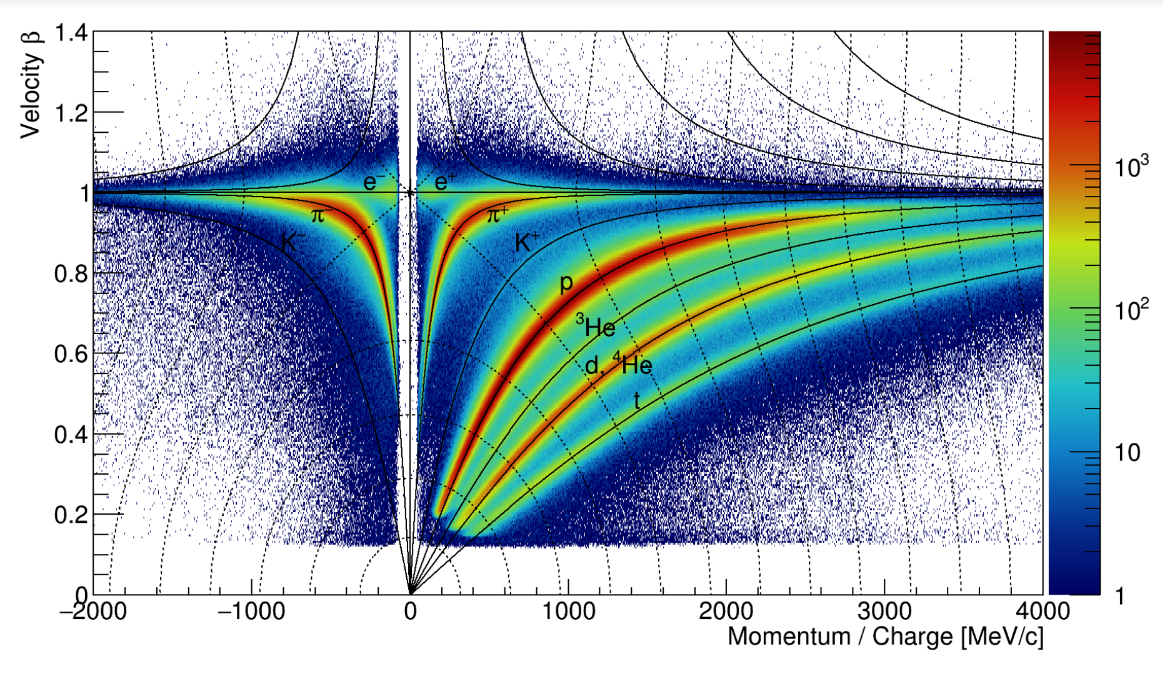
\includegraphics[width=0.95\linewidth]{images/hades_pid_plot.png}
    \caption{Распределение заряженных частиц, зарегистрированных трекинговой системой HADES по относительной скорости $\beta$ и импульсу делённому на заряд $p/q$.}
    \label{fig:hades_pid}
    \end{center}
    \end{figure}
    
Распределение заряженных частиц, зарегистрированных трекинговой системой HADES по квадрату массы $m^2$ и импульсу делённому на заряд $p/q$ представлено на рис.~\ref{fig:hades_m2_pq} (слева).
Ожидается, что массы рожденных частиц, измеренные времяпролётным методом будут распределены согласно нормальному распределению.
Среднее этого распределения для каждого типа частиц не должно зависить от импульса частицы, однако в эксперименте наблюдается сдвиг в сторону меньших значений для протонного пика.
Этот систмематический сдвиг может быть объяснён ошибкой при измерении частиц с малыми импульсами.
Большая кривизна траектории может приводить к ошибкам при ее реконструкции.
Ширина распределения для каждого вида частиц увеличивается с ростом импульса.
Этот эффект объясняется ограниченным разрешением времяпролётной системы, в которой при больших импульсах время пролёта восстанавливается с большей относительной ошибкой.
Каждый из пиков для разных типов частиц аппроксимируется функцией гаусса в узких диапазонах импульса.
Затем на основании этих аппроксимаций происходит отбор кандидатов в частицы для каждого типа.
Отобранные протоны представлены на рис.~\ref{fig:hades_m2_pq} (справа).
%
\begin{figure}[ht]
\begin{center}
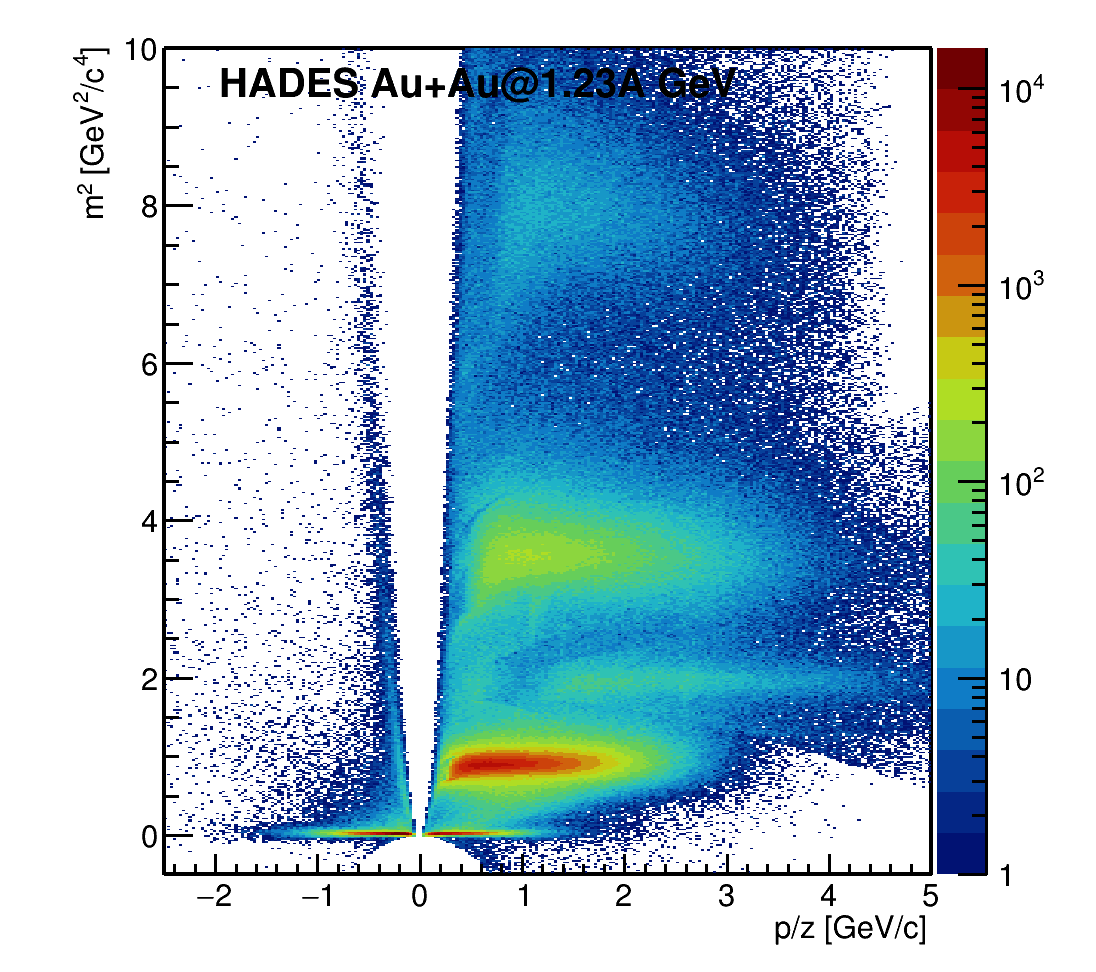
\includegraphics[width=0.45\linewidth]{images/au123_m2_vs_pq_all.png}
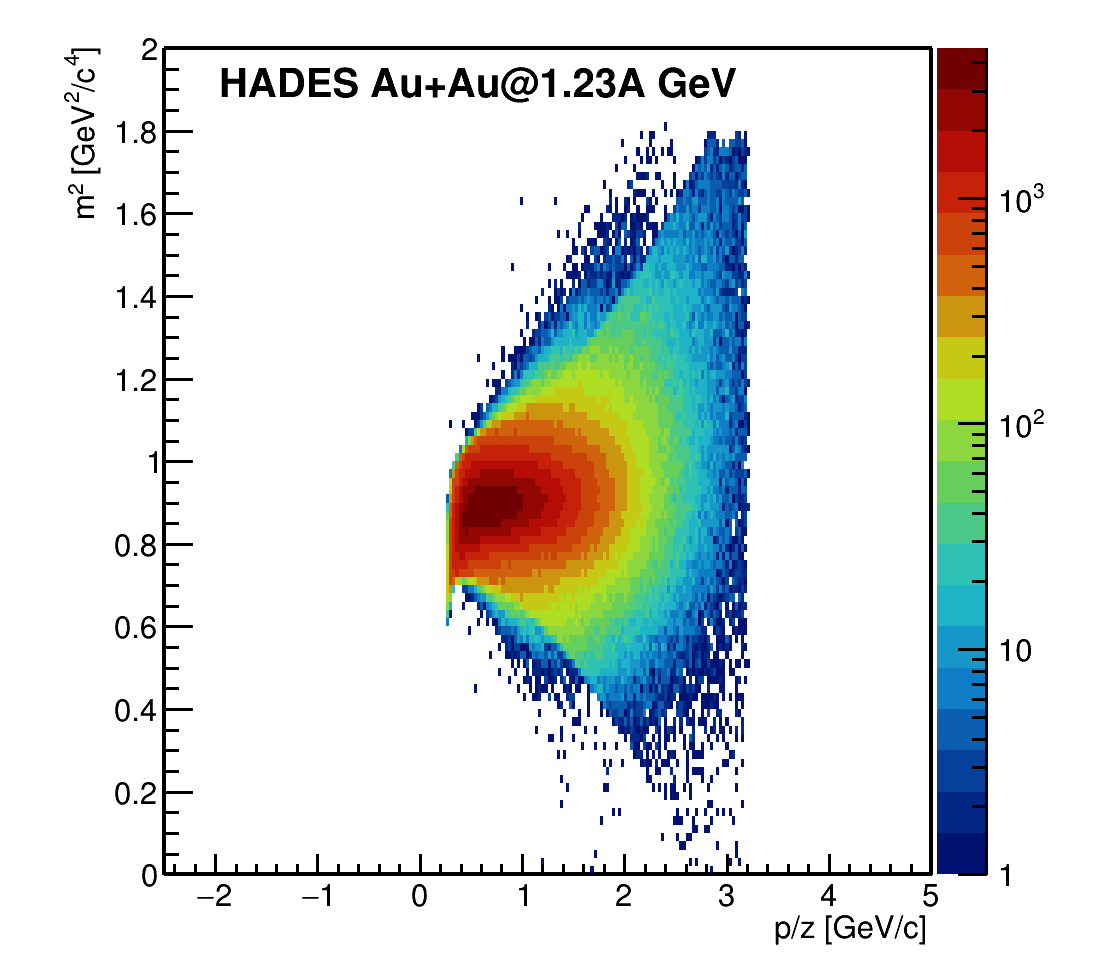
\includegraphics[width=0.45\linewidth]{images/au123_m2_vs_pq_protons.png}
\caption{Распределение заряженных частиц, зарегистрированных трекинговой системой HADES по квадрату массы деленному на квадрат заряда $m^2/q^2$ и импульсу делённому на заряд $p/q$: Для всех заряженных частиц (слева), для отобранных протонов (справа).}
\label{fig:hades_m2_pq}
\end{center}
\end{figure}

\subsection{Кинематические области используемые для определения $Q_1$ векторов}

Оценка плоскости симметрии в работе производилась по асимметрии распределения заряда спектаторов в детекторе FW. 
В качестве веса при вычислении $Q_1$-вектора использовался сигнал, зарегистрированный в модуле.
На рис.~\ref{fig:fw_signal} представлено распределение сигнала в модулях сцинтиляционной стенки FW для столкновений Au + Au при $E_{kin}$=1.23$A$~ГэВ (слева), Ag + Ag при $E_{kin}$=1.23$A$~ГэВ (посередине) и $E_{kin}$=1.58$A$~ГэВ (справа).
Наиболее выраженный пик отвечает заряду $Z=1$ (signal=100).
Также наблюдаются пики для зарядов $Z=2$ и $Z=3$.
События срабатывания модулей стенки с большими зарядами фрагментов редки.
%
\begin{figure}[ht]
\begin{center}
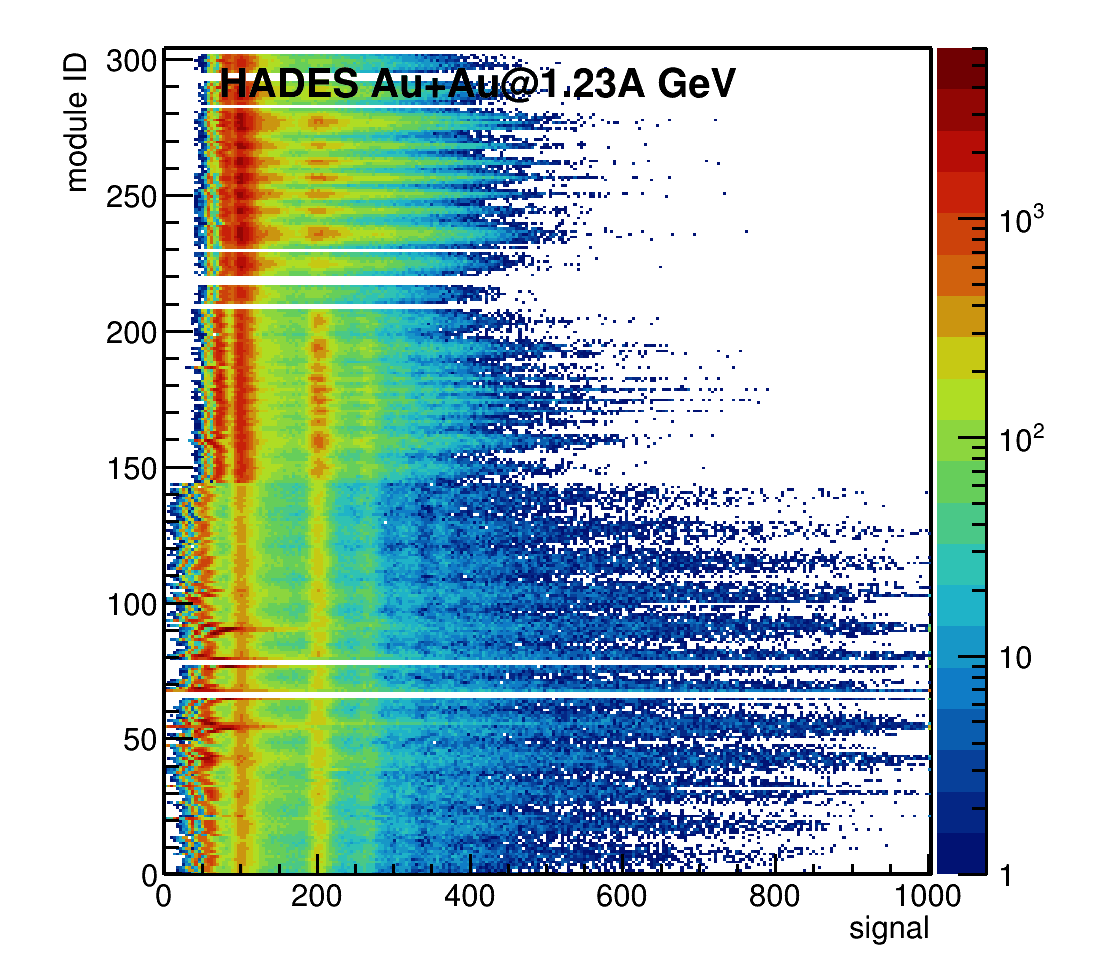
\includegraphics[width=0.3\linewidth]{images/au123_fw_modules.png}
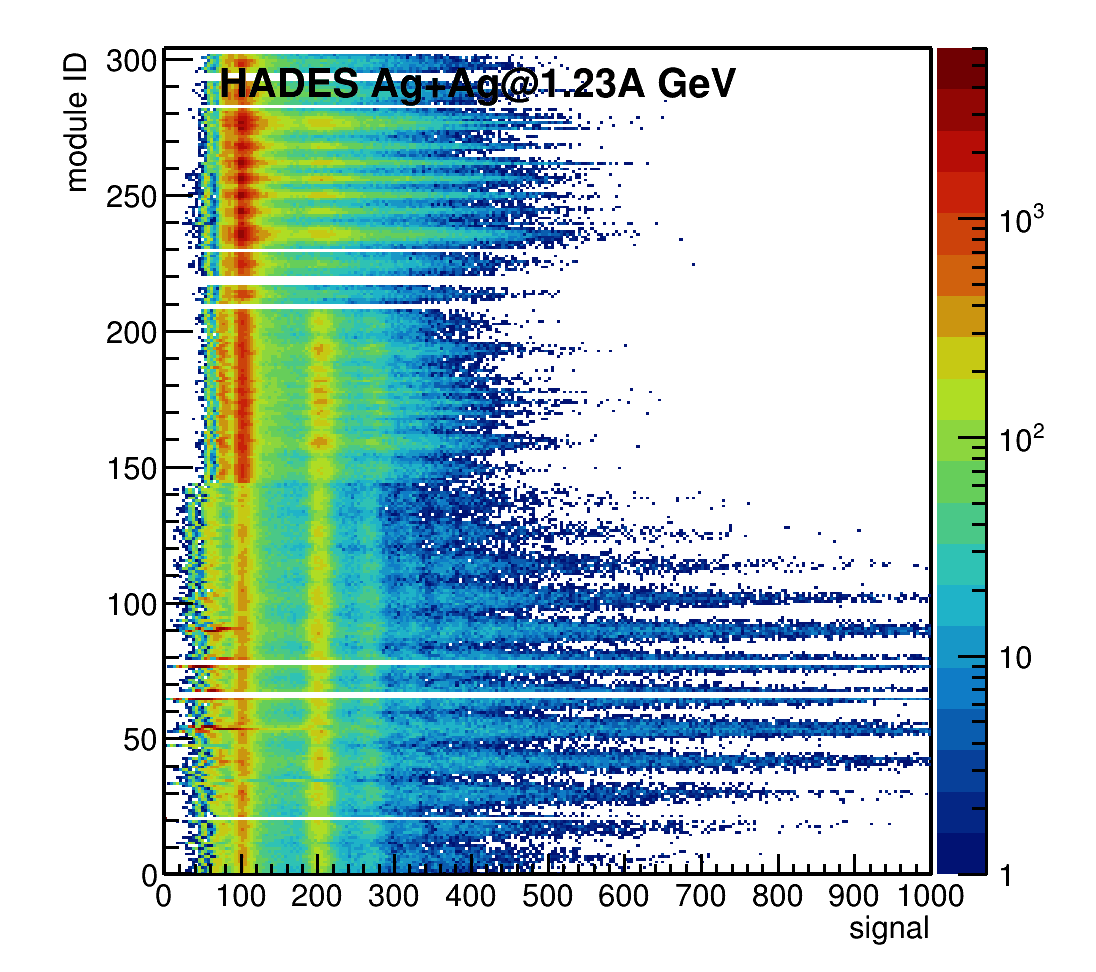
\includegraphics[width=0.3\linewidth]{images/ag123_fw_modules.png}
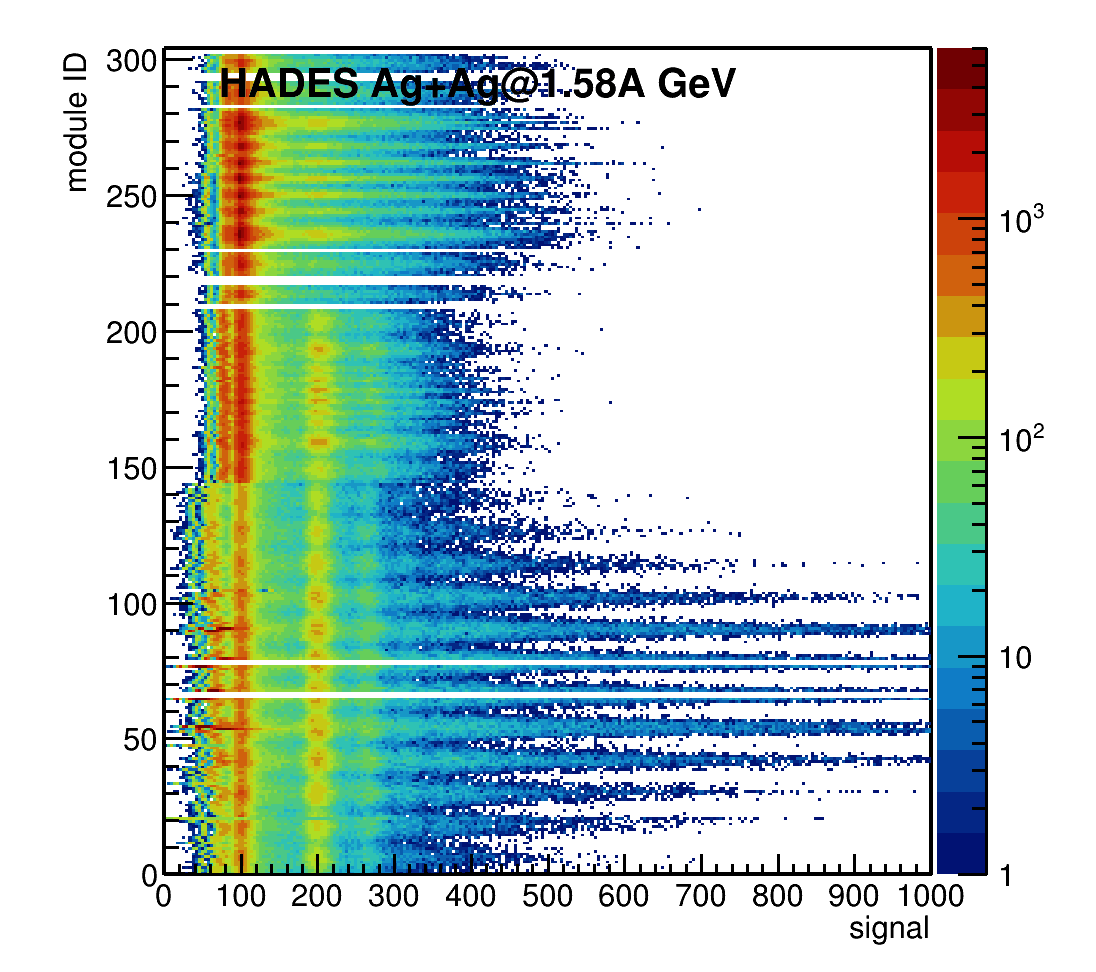
\includegraphics[width=0.3\linewidth]{images/ag158_fw_modules.png}
\caption{Распределение сигнала в модулях сцинтиляционной стенки FW для столкновений Au + Au при $E_{kin}$=1.23$A$~ГэВ (слева), Ag + Ag при $E_{kin}$=1.23$A$~ГэВ (посередине) и $E_{kin}$=1.58$A$~ГэВ (справа). }
\label{fig:fw_signal}
\end{center}
\end{figure}

Для оценки систематической ошибки вызванной непотоковыми корреляциями были введены 2 дополнительных $Q_1$-вектора из треков заряженных частиц.
Векторы $Q_1$ были построены из протонов c поперечным импульсом $p_T < 2.0$~ГэВ с быстротами $0.35 < y_{cm} < 0.55$ (Mf) и $-0.55 < y_{cm} < -0.35$ (Mb).
Модули детектора FW были разделены на 3 группы: центральные (W1), средние (W2) и периферические (W3).
Схематически расположение полученных векторов в плоскости $\eta$-$p_T$ изображено на рис~\ref{fig:hades_qvectors}.
%
\begin{figure}[ht]
\begin{center}
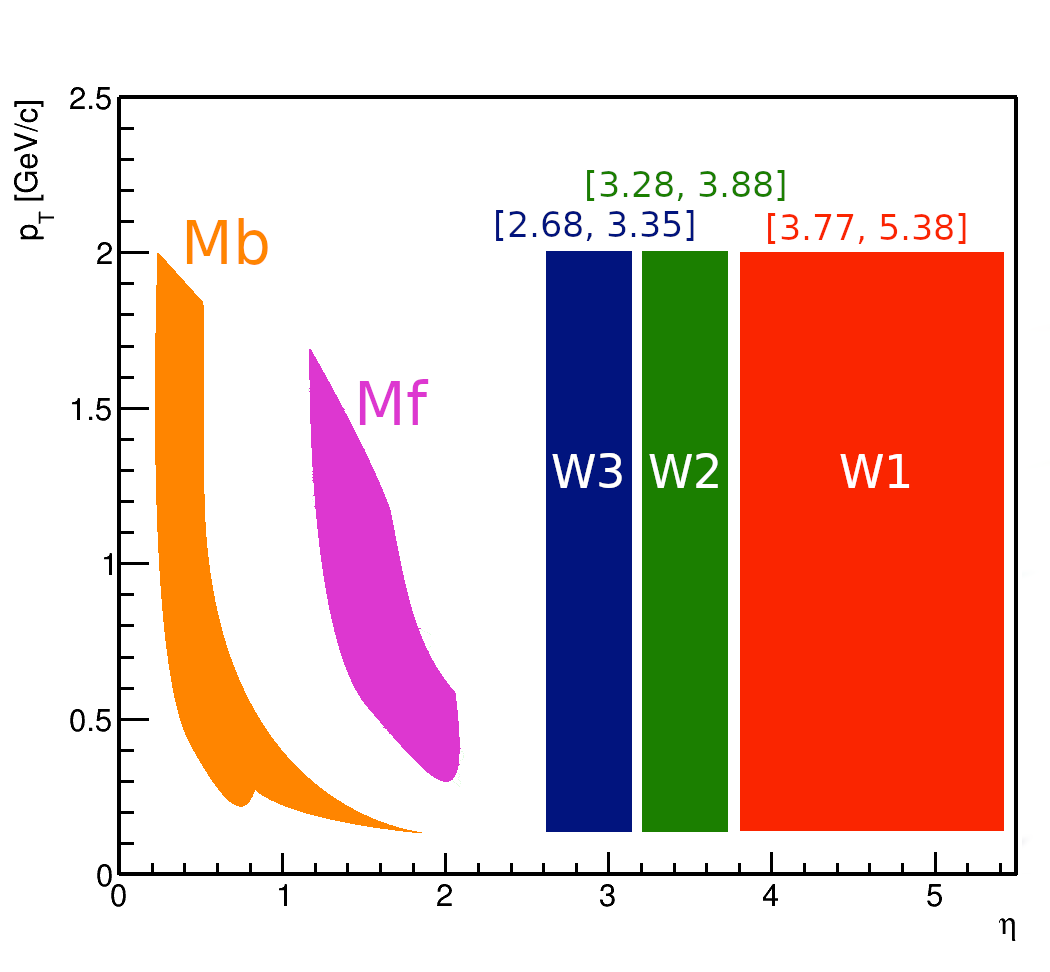
\includegraphics[width=0.75\linewidth]{images/eta_pt_qvectors.png}
\caption{Aксептанс по псевдобыстроте $\eta$ для подсобытий из FW и поперечному импульсу $p_T$ для подсобытий из MDC, использованных для расчета направленного потока протонов в столкновениях ядер золота и серебра.}
\label{fig:hades_qvectors}
\end{center}
\end{figure}
%

\subsection{Коррекция азимутальной анизотропии аксептанса детектора}

Азимутальный аксептанс трекинговой системы в зависимости от быстроты частицы приведён на рис.~\ref{fig:hades_phi_y}.
Азимутальный аксептанс трекинговой системы не является однородным, поскольку стыки секций трекинговой системы не способны регистрировать заряженные частицы.
Неоднородность увеличивается с ростом быстроты, поскольку площадь нечувствительного объёма по отношению к чувствительному уменьшаяется с ростом полярного угла $\theta$. 
%
\begin{figure}[ht]
\begin{center}
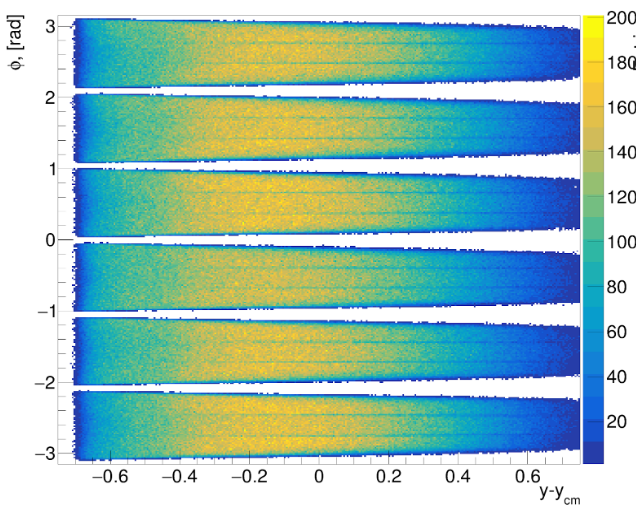
\includegraphics[width=0.55\linewidth]{images/hades_phi_y.png}
\caption{Азимутальный аксептанс трекинговой системы эксперимента HADES в зависимости от быстроты частицы.}
\label{fig:hades_phi_y}
\end{center}
\end{figure}

Для коррекции азимутальной неоднородноссти аксептанса был использован метод, предложенный в~\cite{Selyuzhenkov:2007zi}.
Данный метод основан на предположении, что азимутальное распределение частиц, рожденных в столкновении должно быть изотропным, поскольку угол плоскости реакции от события к событию распределен равномерно.
Азимутальная неоднородность чувствительного объема детектора вносит искажения в азимутальное распределение зарегистрированных частиц. 
Для коррекции на этот эффект, в статье~\cite{Selyuzhenkov:2007zi} вводятся поправки перецентровки, поворота и ремасштабирования. 
Схематически, действие этих поправок представлено на рис.~\ref{fig:qn_corrections}.
%
\begin{figure}[ht]
\begin{center}
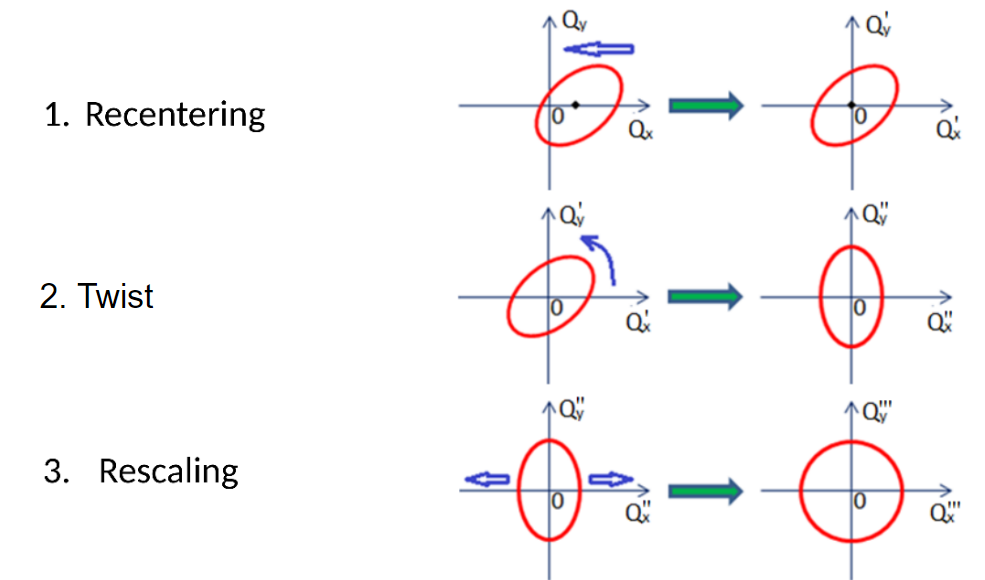
\includegraphics[width=0.75\linewidth]{images/qntools_corrections.png}
\caption{Схематическое изображение поправок предложенных в~\cite{Selyuzhenkov:2007zi}.}
\label{fig:qn_corrections}
\end{center}
\end{figure}
%

Описанные выше поправки применялись для коррекции азимутальной неоднородности аксептанса детектора мультидифференциально.
Для $Q_1$-векторов коррекции применялись в каждом классе центральности от 0\% до 40\% с шагом 5\%.
Для поправок на азимутальную неоднородность трекинга, коррекции на $u_1$-вектор применялись аналогично в каждом классе центральности а также дифференциально по поперечному импульсу $p_T$ и быстроте $y_{cm}$. 
Остаточные эффекты азимутальной неоднородности аксептанса в данной работе оцениваются как разность между корреляцией компонент $u_1$ и $Q_1$-векторов:
\begin{equation}
    \delta_{acc.} = | \langle x_1 X_1 \rangle - \langle y_1 Y_1 \rangle |,
\end{equation}
где $\delta_{acc.}$ --- остаточная ошибка после применения коррекций, $x_1$ и $y_1$, и $X_1$ и $Y_1$ --- компоненты $u_1$ и $Q_1$-векторов соответственно. 

Сравнение $v_1^{uncorr.}$, полученного с использованием различных компонент $u_1$ и $Q_1$-векторов, представлено на рис~\ref{fig:hades_uq_corr}. 
Направленный поток не корректирован на разрешение плоскости симметрии для оценки вклада неоднородного аксептанса трекинговой системы. 
После применения поправок на азимутальную анизотропию аксептанса, остаточный эффект составляет 2\%.
%
\begin{figure}[ht]
\begin{center}
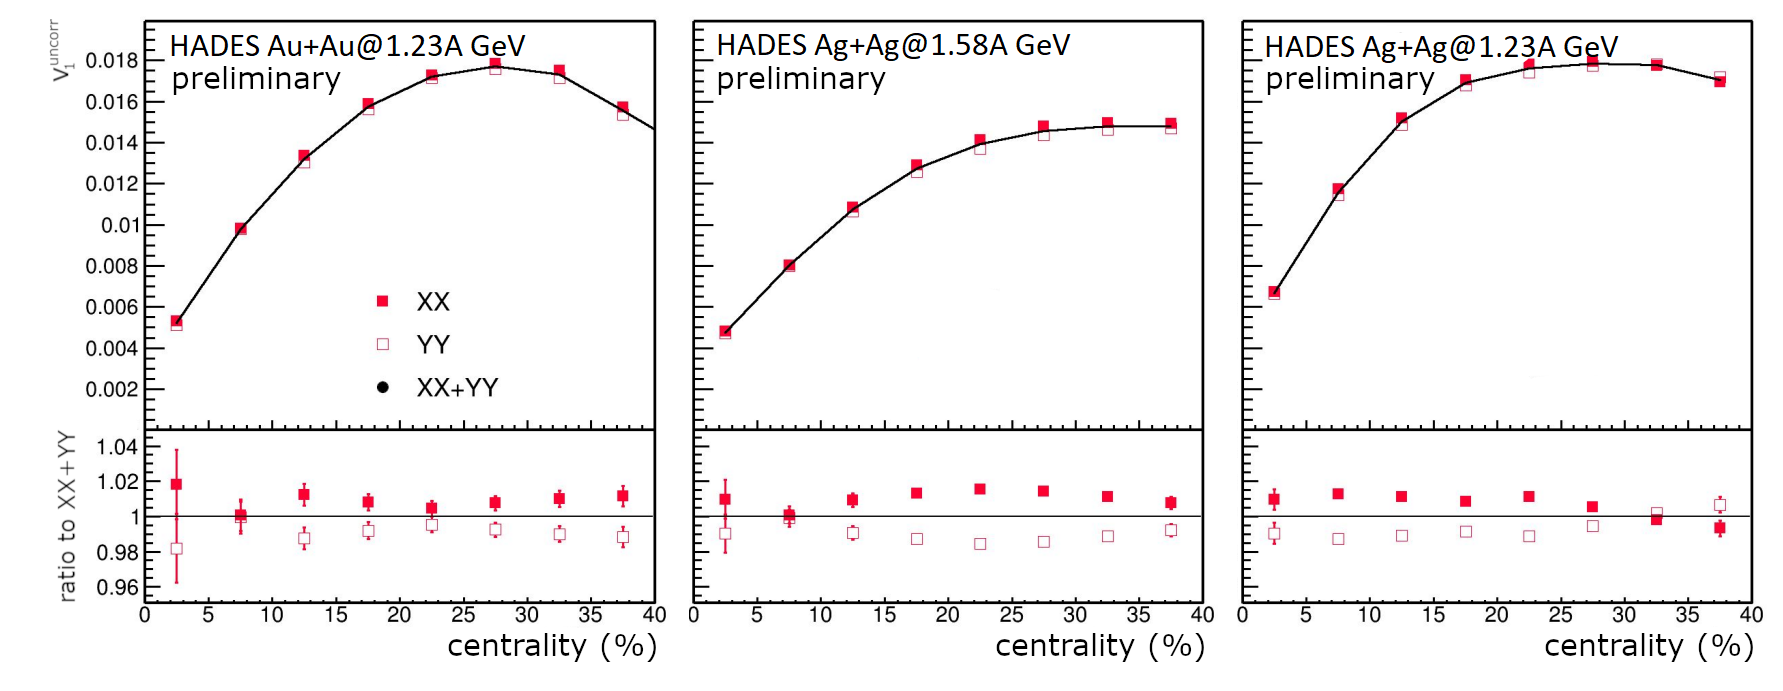
\includegraphics[width=0.75\linewidth]{images/hades_u1W1_centrality.png}
\caption{Сравнение компонент корреляции $\langle u_1 Q_1 \rangle$ после применения поправок на азимутальную неоднородность детектора для столкновений Au+Au@1.23A ГэВ (слева), Ag+Ag@1.23A ГэВ (посередине) и Ag+Ag@1.58A ГэВ (справа)}
\label{fig:hades_uq_corr}
\end{center}
\end{figure}
%

\subsection{Вычисление поравочного коэффициента разрешения $R_1$}

Для рассчета разрешения методом случайных подсобытий два вектора были определены из модулей детектора FW.
Модули были распределены в две группы случайным образом для каждого события.
На рис.~\ref{fig:hades_R1_rs} представлено разрешение плоскости симметрии рассчитанное методом случайных подсобытий как функция центральности столкновения.
Основным недостатком данного метода является отсутствие возможности сравнить полученные значения с другими оценками разрешения плоскости симметрии.
%
\begin{figure}[ht]
\begin{center}
    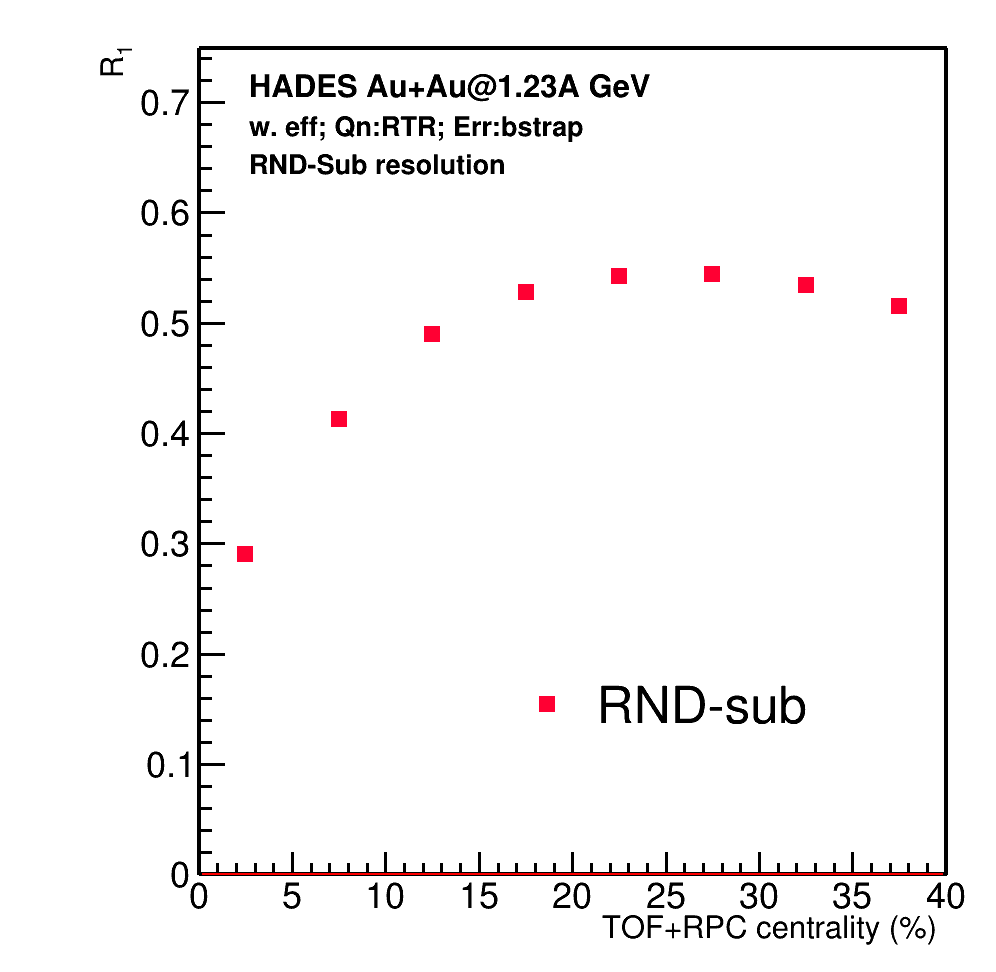
\includegraphics[width=0.3\linewidth]{images/R1_au123_rnd_centrality.png}
    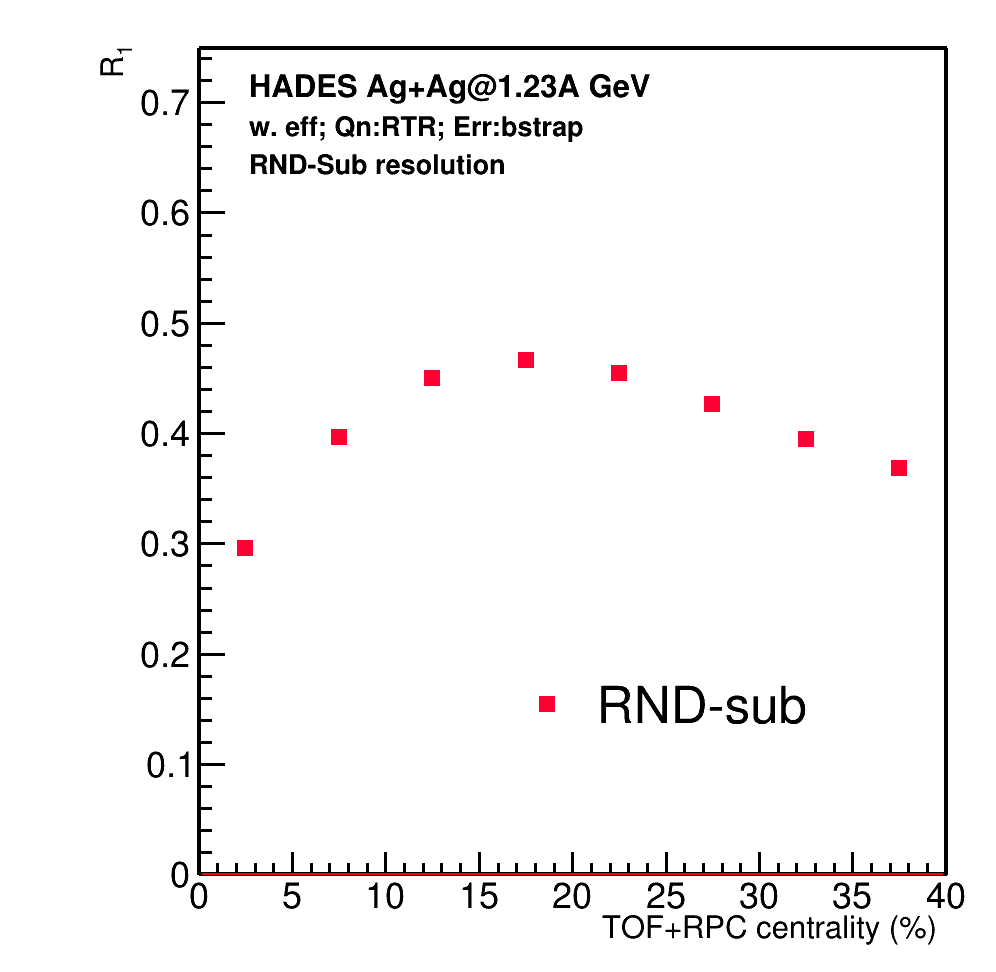
\includegraphics[width=0.3\linewidth]{images/R1_ag123_rnd_centrality.png}
    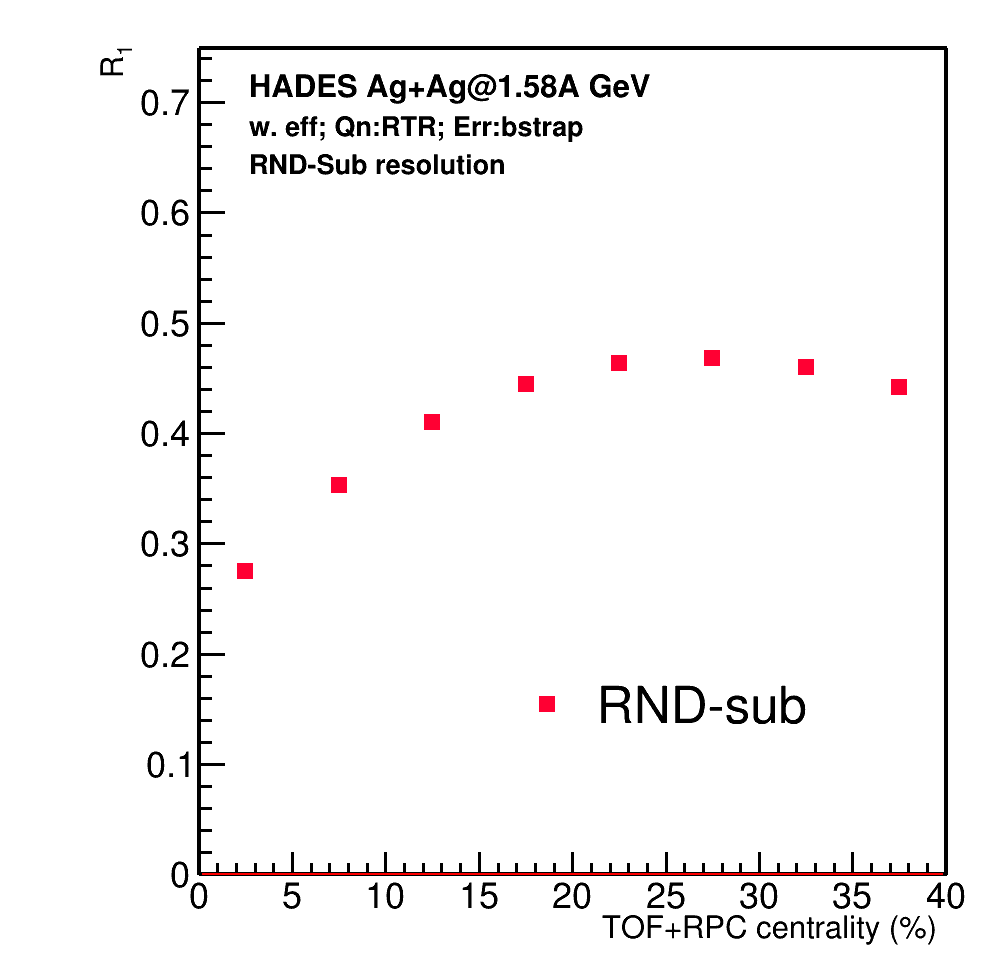
\includegraphics[width=0.3\linewidth]{images/R1_ag158_rnd_centrality.png}
    \caption{Разрешение плоскости симметрии рассчитанное методом случайных подсобытий как функция центральности столкновения.
    Слева: для столкновений Au + Au при $E_{kin}$=1.23$A$~ГэВ;
    посередине: для столкновений Ag + Ag при $E_{kin}$=1.23$A$~ГэВ; 
    справа: для столкновений Ag + Ag при $E_{kin}$=1.58$A$~ГэВ; 
    }
    \label{fig:hades_R1_rs}
\end{center}
\end{figure}
%

Для расчета разрешения методом трёх подсобытий в работе введены 5 $Q_1$-векторов. 
Используя в методе трех подсобытий различные комбинации векторов, можно оценить остаточные эффекты из-за непотоковых корреляций. 
Очевидно, что разрешение плоскости симметрии, посчитанное с использованием различных комбинаций, должны совпадать, а возможная разница будет связана с эффектами не относящимися к коллективному движению частиц.
Исключая из анализа разрешение полученное при помощи комбинаций, в которых два или более векторов коррелируют по непотоковому каналу, можно значительно уменьшить вклад непотоковых корреляций в полученные результаты.
Таким образом, систематическая ошибка из-за эффектов, не связанных с коллективным движением частиц может быть рассчитана следующим образом:
\begin{equation}
    \delta_{NF} = R_1\{a(b,c)\} - R_1\{d(e,f)\},
\end{equation}
где $\delta_{NF}$ --- ошибка из-за непотоковых корреляций, а буквами от $a$ до $f$ обозначены различные $Q_1$-вектора.

Разрешение плоскости симметрии $W1$, полученное с использованием различных комбинаций $Q_1$-векторов, показано на рис~\ref{fig:hades_w1_combinations}.
Разрешение $R_1\{W1(W2,W3)\}$ заметно отличается от значений, полученных при помощи других комбинаций. 
Этот эффект может быть объяснён наличием непотоковых корреляций между парами $Q_1$-векторов $W1$ и $W2$, $W2$ и $W3$.
Эти векторы не имеют достаточного разделения по быстроте, поэтому в значительной степени могут быть подвержены непотоковым корреляциям. 
В столкновениях Ag+Ag при обеих энергиях, $R_1\{W1(Mf,Mb)\}$ также значительно отклоняется от среднего результата. 
Это может быть вызвано наличием корреляций из-за закона сохранения импульса между векторами $Mf$ и $Mb$. 
В столкновениях Au+Au этот эффект менее выражен в силу большей множественности рождённых частиц.
%
\begin{figure}[ht]
\begin{center}
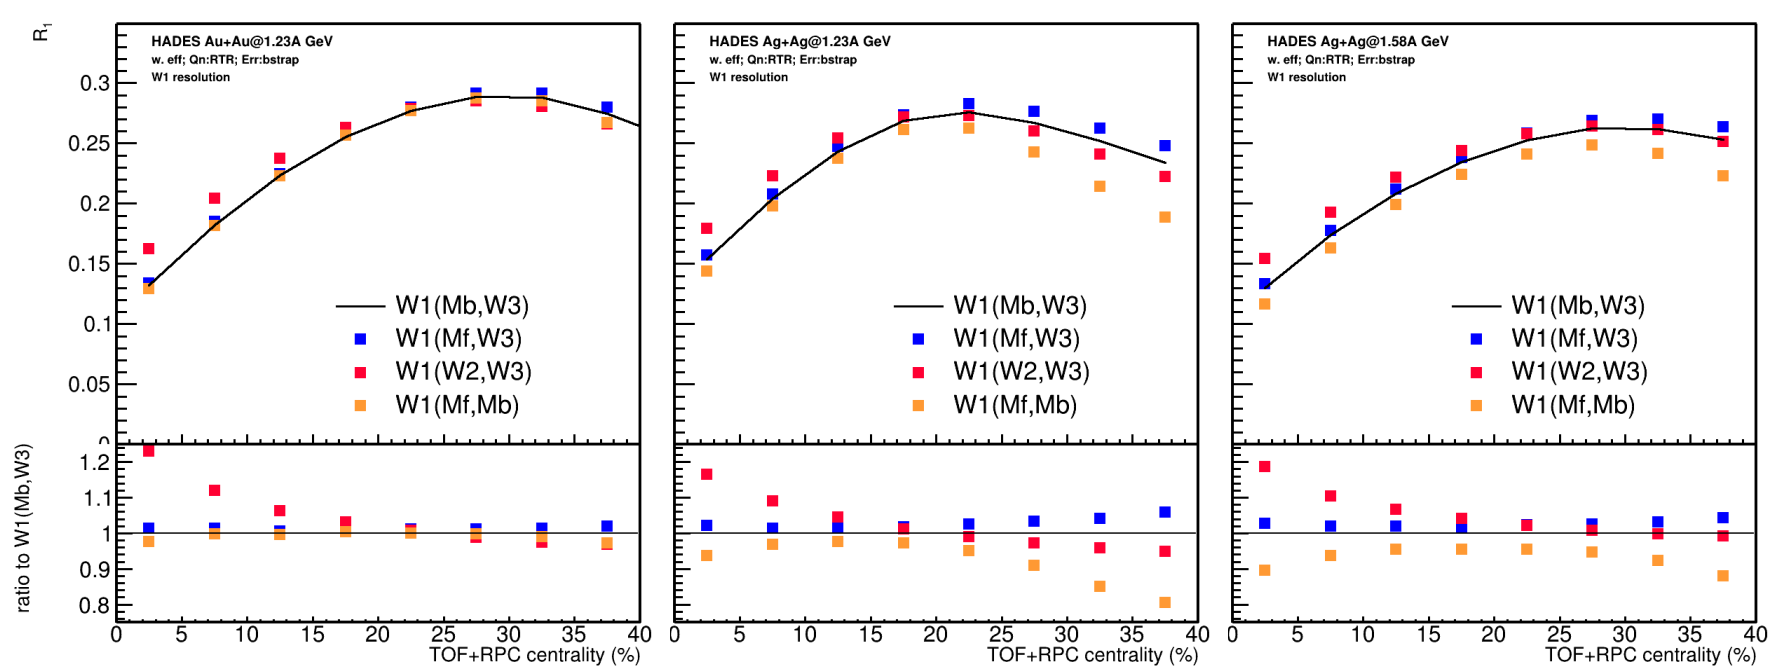
\includegraphics[width=0.75\linewidth]{images/W1_combinations.png}
\caption{Сравнение разрешений плоскости симметрии $W1$ полученное с использованием различных комбинаций $Q_1$-векторов для Au+Au@1.23A ГэВ (слева), Ag+Ag@1.23A ГэВ (посередине) и Ag+Ag@1.58A ГэВ (справа)}
\label{fig:hades_w1_combinations}
\end{center}
\end{figure}

\section{Эксперимент BM@N}

\subsection{Моделирование отклика установки}

Разработанная физическая программа измерения коллективных потоков в эксперименте BM@N была проверена на реалистичном Монте-Карло моделировании отклика детектора. 
В качестве входных данных моделирования были использованы две физические модели столкновения тяжелых ионов.
Модель DCM-QGSM-SMM (Dubna Cascade Model, Quark-Gluon String Model, Statistical Multifragmentation Model)~\cite{Botvina:1994vj,Baznat:2019iom} реалистично описывает выход спектаторных фрагментов, однако неудовлетворительно воспроизводит коллективную анизотропию рожденных частиц.
Эта модель была использована для проверки разработанных методов вычисления поправочного коэффициента разрешения в эксперименте BM@N.

Модель JAM (Jet-A-A Model)~\cite{Nara:2016hbg,Nara:2019qfd,Nara:2020ztb} с импульсно-зависимым потенциалом дает реалистичный сигнал коллективной анизотропии рожденных барионов, однако в модели отсутствуют фрагменты с массовым номером $A>1$.
Данная модель была использована для проверки коррекций на неоднородность детектора и возможности алгоритмов реконструкции восстановить сигнал коллективной анизотропии.

В плоскости поперечной направлению пучка аксептанс установки имеет прямоугольную форму, что ведёт к значительной неоднородности аксептанса.
На рис.~\ref{fig:bmn_phi_eta} представлен азимутальный аксептанс заряженных частиц в зависимости от псевдобыстроты. 
%
\begin{figure}[ht]
\begin{center}
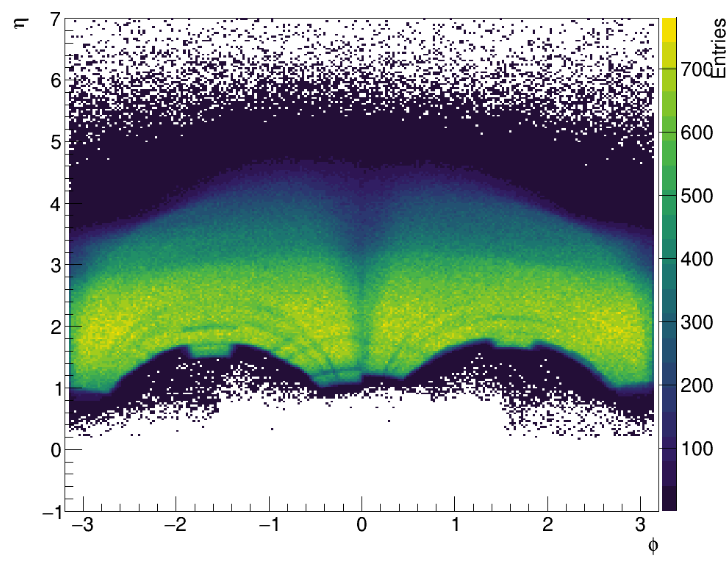
\includegraphics[width=0.55\linewidth]{images/bmn_phi_eta.png}
\caption{Азимутальный аксептанс заряженных частиц в зависимости от псевдобыстроты.}
\label{fig:bmn_phi_eta}
\end{center}
\end{figure}

На рис.~\ref{fig:bmn_mom_res} показано импульсное разрешение трекинговой системы как функция импульса частицы.
Различными цветами и маркерами показаны различные энергии столкновения ядер Xe и Cs.
Разрешение падает с уменьшением энергии столкновения. 
Этот эффект связан с уменьшением магнитного поля, при уменьшении энергии столкновения. 
При энергии $E_{kin}$=2$A$~ГэВ, экспериментальная установка работает с магнитным полем 0.4~Тл, при энергии $E_{kin}$=3$A$~ГэВ магнитное поле 0.6~Тл и при энергии $E_{kin}$=4$A$~ГэВ --- 0.8~Тл.
%
\begin{figure}[ht]
\begin{center}
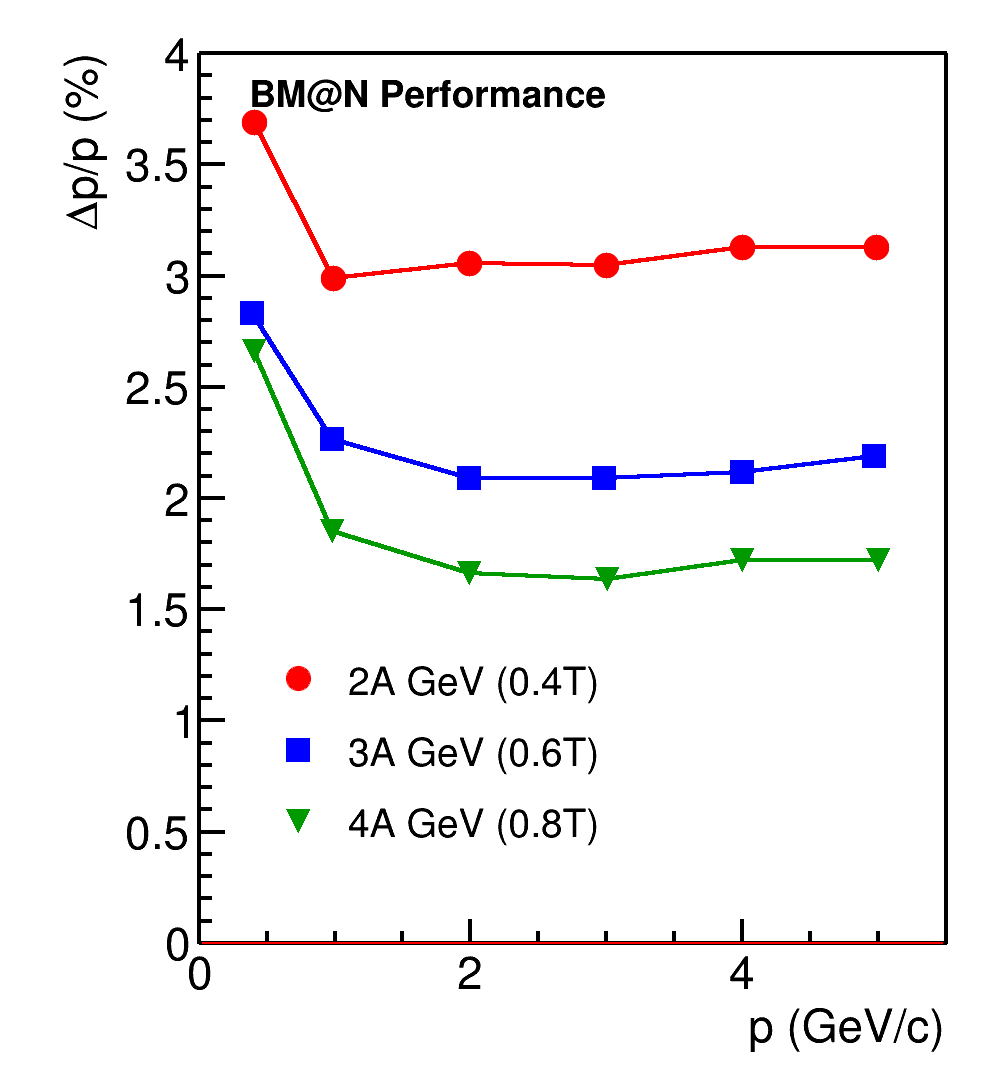
\includegraphics[width=0.55\linewidth]{images/momentum_resolution.png}
\caption{Разрешение трекинговой системы по импульсу в эксперименте BM@N. Различными цветами и маркерами показана различная энергия столкновения.}
\label{fig:bmn_mom_res}
\end{center}
\end{figure}

\subsection{Определение центральности}

В эксперименте BM@N центральность была определена при помощи метода Монте-Карло Глаубера, в качестве множественности использовалось число восстановленных траекторий заряженных частиц~\cite{Segal:2023njv}.
В качестве параметров распределения Вудса-Саксона (\ref{eq:woods_saxon}) использовались следющие значения: Xe ($A=129$, $Z=54$, $R=5.46$~фм, $a=0.57$~фм) и Cs ($A=133$, $Z=55$, $R=6.125$~фм, $a=0.5$~фм).
Далее согласно процедуре, описанной в секции~\ref{theory:centrality}, были разыграны параметры $N_{part}$, $N_{col}$ и путем варьирования $f$, $\mu$ и $k$ достигалось наилучшее согласие смоделированной множественности с экспериментальной.
Восстановленное методом МК-Глаубера распределение множественности при полном сечении неупругого взаимодействия было разбито на классы центральности по 5\% и 10\%.

На рис.~\ref{fig:bmn_multiplicity} слева представлено распределение множественности заряженных частиц для Монте-Карло моделирования столкновений Xe+Cs(I) при энергии $E_{kin}$=4$A$~ГэВ.
Открытыми маркерами обозначено распределение множественности заряженных траекторий после полной цепочки реконструкции событий модели DCM-QGSMSMM.
Синими треугольниками представлено распределение множественности полученное методом МК-Глаубра.
Вертикальными линиями обозначены границы классов центральности.
Модель Монте-Карло Глаубера хорошо описывает распределение множественности в границах 0-80\% класса центральности.
Справа представлены значения среднего прицельного параметра в каждом классе центральности по множественности.
Открытые символы обозначают значения, полученные из модели DCM-QGSMSMM.
Синие треугольники --- значение, извлеченные из модели МК-Глаубера.
Наблюдается хорошее согласие между реконструированными значениями прицельного параметра и настоящими из DCM-QGSMSMM.
%
\begin{figure}[ht]
\begin{center}
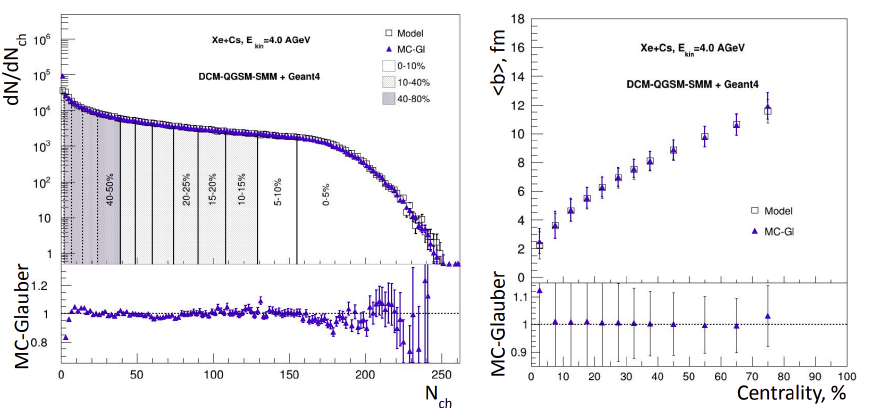
\includegraphics[width=0.95\linewidth]{images/mc_glauber_xecs_mult.png}
\caption{Слева: распределение множественности заряженных частиц в эксперименте BM@N. Вертикальными линиями изображены границы классов центральности. Справа: значения среднего прицельного параметра в классах центральности, определенных по множественности.}
\label{fig:bmn_multiplicity}
\end{center}
\end{figure}

\subsection{Идентификация протонов}

Для каждого из детекторов была построена зависимость квадрата массы делённого на квадрат заряда $m^2/q^2$ от импульса $p/q$. 
На рис.~\ref{fig:bmn_m2_pq} сверху, представлено распределение квадрата массы заряженной частицы в зависимости от импульса $p/q$ для TOF-400 (слева) и TOF-700 (справа).
В узких диапазонах поперечного импульса распределение частиц по квадрату массы было аппроксимировано гауссовой функцией. 
На рис.~\ref{fig:bmn_m2_pq} снизу, представлены кандидаты в протоны, которые лежат не дальше $2\sigma$ от пика квадрата массы.
%
\begin{figure}[ht]
\begin{center}
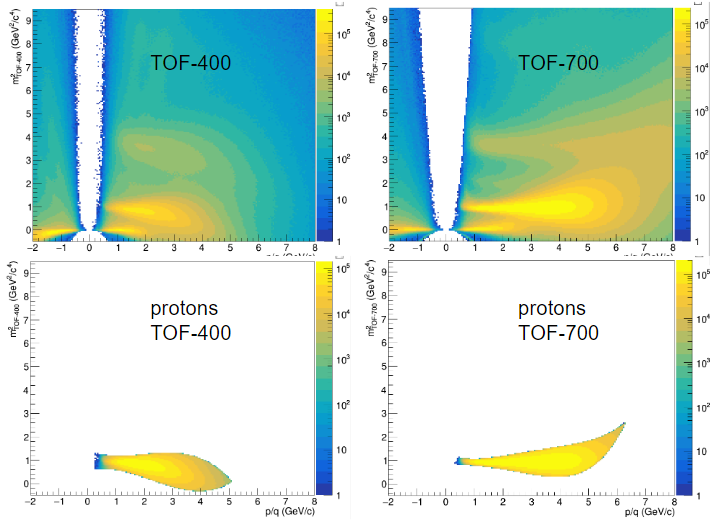
\includegraphics[width=0.95\linewidth]{images/bmn_m2_pq.png}
\caption{Распределение квадрата массы деленного на квадрат заряда заряженной частицы в зависимости от импульса $p/q$ для TOF-400 (слева) и TOF-700 (справа). Сверху представлены распределения для всех заряженных частиц, снизу --- для отобранных протонов.}
\label{fig:bmn_m2_pq}
\end{center}
\end{figure}


На рис.~\ref{fig:bmn_pt_y} представлено распределение протонов по быстроте $y_{cm}$ и поперечному импульсу $p_T$ идентифицированных при помощи TOF-400 (слева сверху), TOF-700 (слева снизу), с использованием обоих TOF-детекторов (справа).
%
\begin{figure}[ht]
\begin{center}
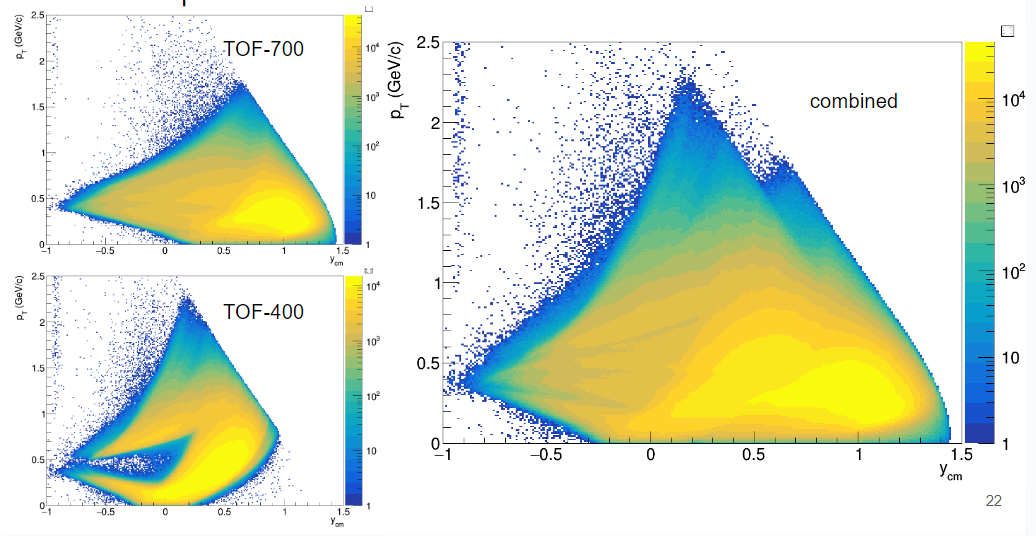
\includegraphics[width=0.95\linewidth]{images/bmn_pt_y_acceptance.png}
\caption{Распределение протонов по быстроте $y_{cm}$ и поперечному импульсу $p_T$, идентифицированных при помощи TOF-400 (слева сверху), TOF-700 (слева снизу), с использованием обоих TOF-детекторов (справа).}
\label{fig:bmn_pt_y}
\end{center}
\end{figure}


\subsection{Кинематические окна, в которых были определены $Q_1$-вектора}

Для восстановления плоскости симметрии в эксперименте BM@N была использована информация с калориметра FHCal.
Модули детектора были разделены на 3 группы согласно их псевдобыстроте (F1, F2 и F3).
Схематические группы модулей изображены различными цветами на рис.~\ref{fig:bmn_subevents} слева.

Дополнительно для исследования вклада непотоковых корреляций в измеренные значения коллективной анизотропии были введены два $Q_1$-вектора из треков заряженных частиц. 
Вектор $Tp$ построен для протонов со значениями быстроты $0.4<y_{cm}<0.6$ и поперечным импульсом $0.2<p_{T}<2.0$~$GeV/c$.
Вектор $T\pi$ формировался для отрицательных пионов с быстротой и поперечным импульсом $0.2<y_{cm}<0.8$ и $0.1<p_T<0.5 GeV/c$ соответственно.
Соответствующие кинематические области изображены красными прямоугольниками на рис.~\ref{fig:bmn_subevents} справа.
%
\begin{figure}[ht]
\begin{center}
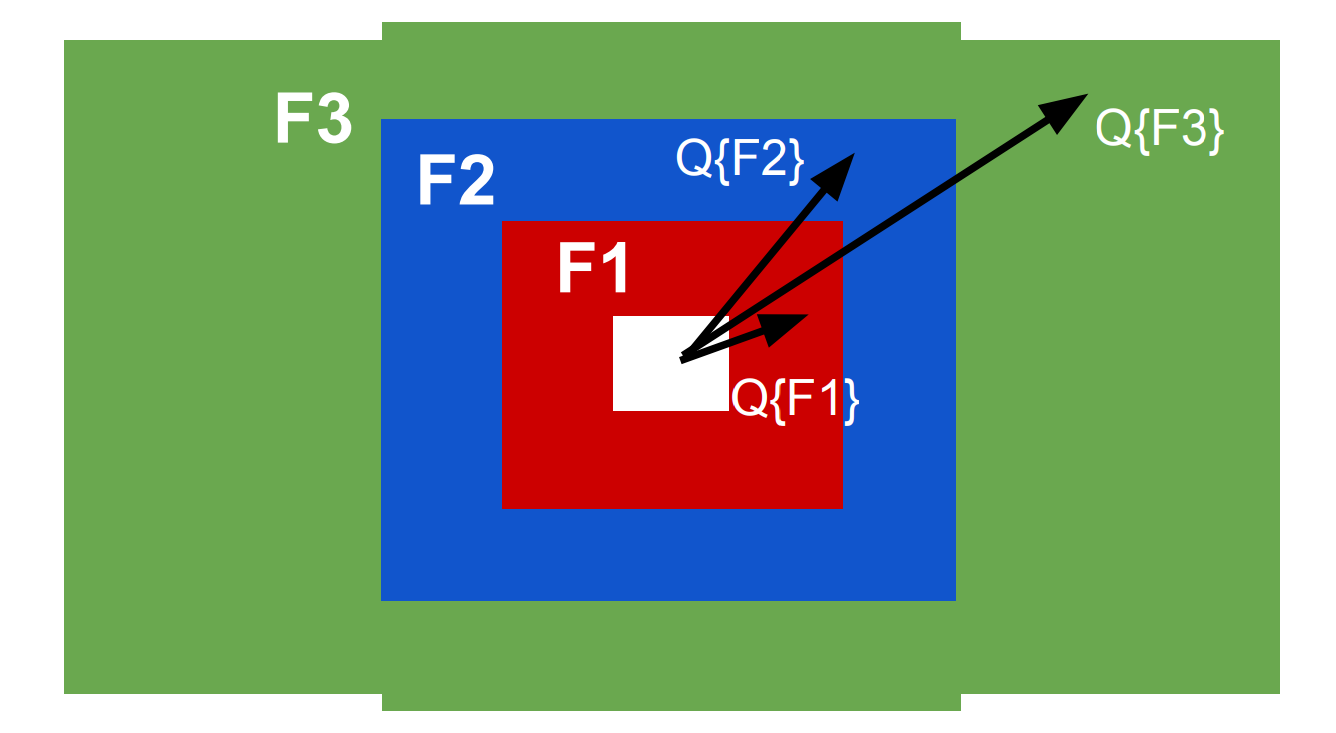
\includegraphics[width=0.45\linewidth]{images/FHCal_layout.png}
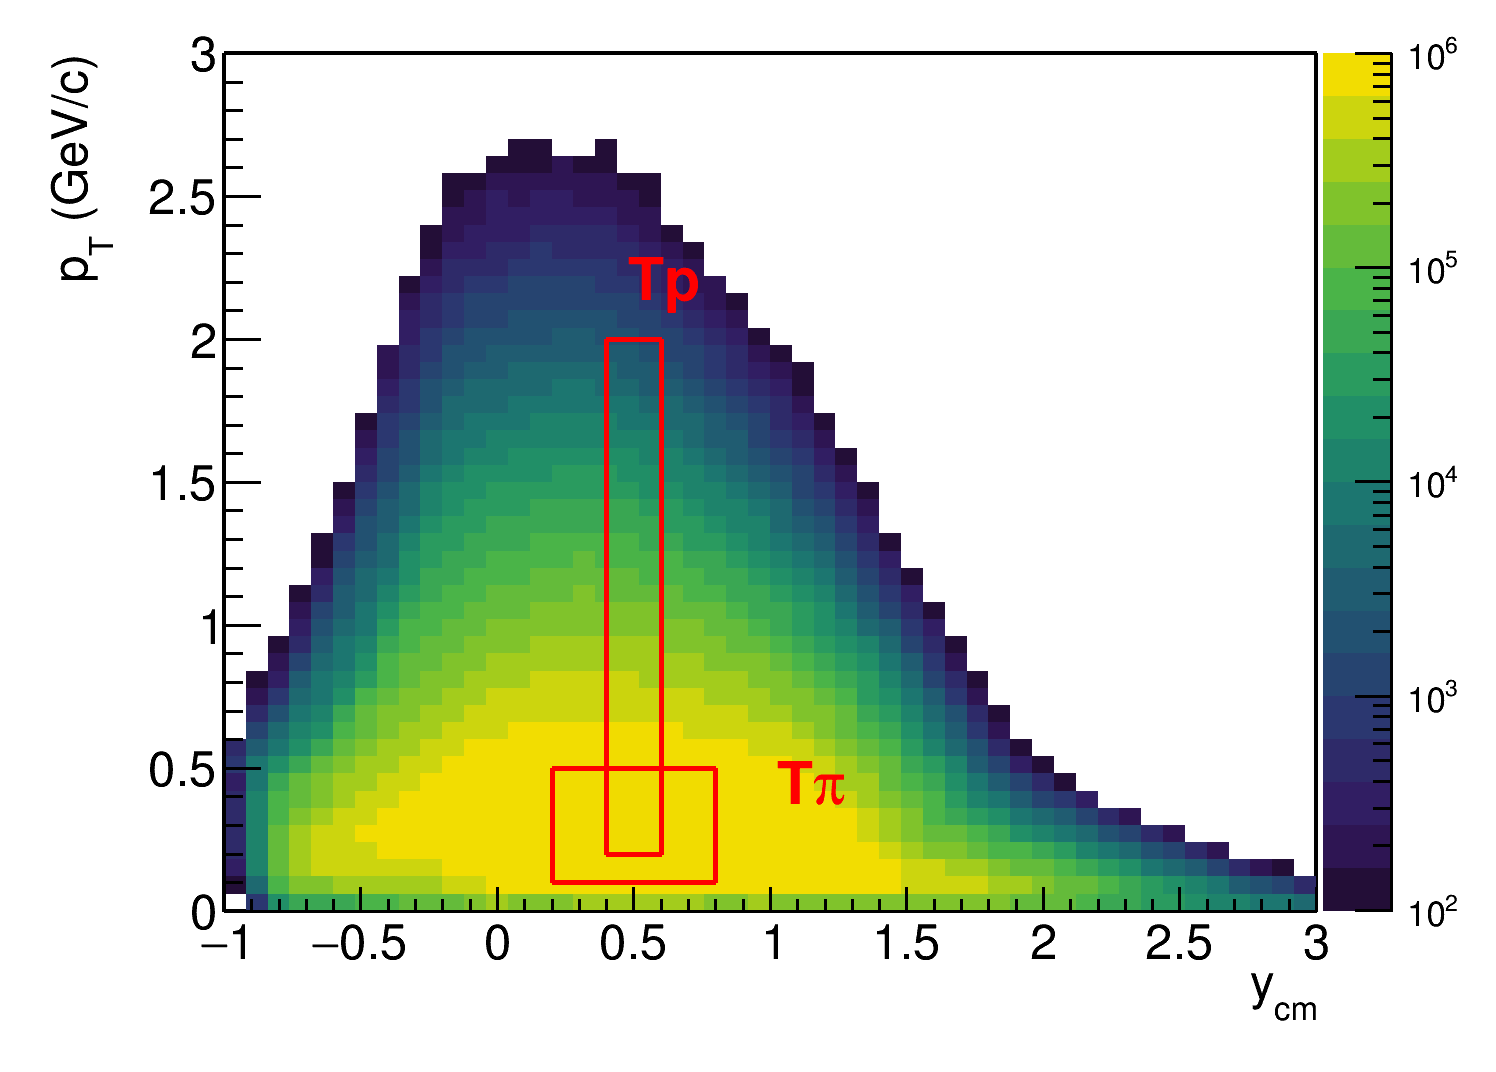
\includegraphics[width=0.45\linewidth]{images/pT_ycm_protons.png}
\caption{
Слева: Схема разделения модулей переднего адронного калориметра по группам для определения плоскости симметрии события.
Справа: Кинематические окна для подсчета $Q_1$-векторов из треков заряженных частиц.
}
\label{fig:bmn_subevents}
\end{center}
\end{figure}

\section{Выводы к главе 3}

В главе описаны методы определения центральности и идентификации протонов с помощью экспериментальной установки HADES.
Представлены критерии отбора столкновений Au+Au и Ag+Ag а также заряженных частиц, рожденных в этих столкновениях.
Описаны способы вычисления эффективности реконструкции протонов при помощи программного пакета GEANT3.
В главе обсуждаются методы определения плоскости симметрии столкновения а также способы вычисления разрешения плоскости симметрии при помощи переднего годоскопа FW в эксперименте HADES.
Приводятся результаты применения коррекций на азимутальную анизотропию аксептанса установки HADES и обсуждаются остаточные систематические погрешности, связанные с этим эффектом.

Для экспериментальной установки BM@N описываются методы измерения центральности столкновения по числу треков заряженных частиц. 
В главе обсуждаются способы измерения производительности установки BM@N для измерения направленного и эллиптического потоков протонов с помощью физических Монте-Карло моделей столкновений тяжелых ионов и программного пакета GEANT4.
В главе представлены значения поправочного коэффициента разрешения $R_1$ для плоскостей симметрии, определенных при помощи переднего годоскопа FW.
Обсуждаются методы минимизации систематической ошибки связанной с непотоковыми корреляциями и вычисляется остаточная систематическая ошибка.
В главе представлены кинематические диапазоны, использованные для вычисления $Q_1$-векторов в Монте-Карло симуляции эксперимента BM@N.